
\section{Langkah-Langkah Percobaan}


\begin{enumerate}

    \item Akses router melalui Winbox menggunakan MAC address dan lakukan reset konfigurasi ke pengaturan awal.
      \begin{figure}[H]
        \centering
        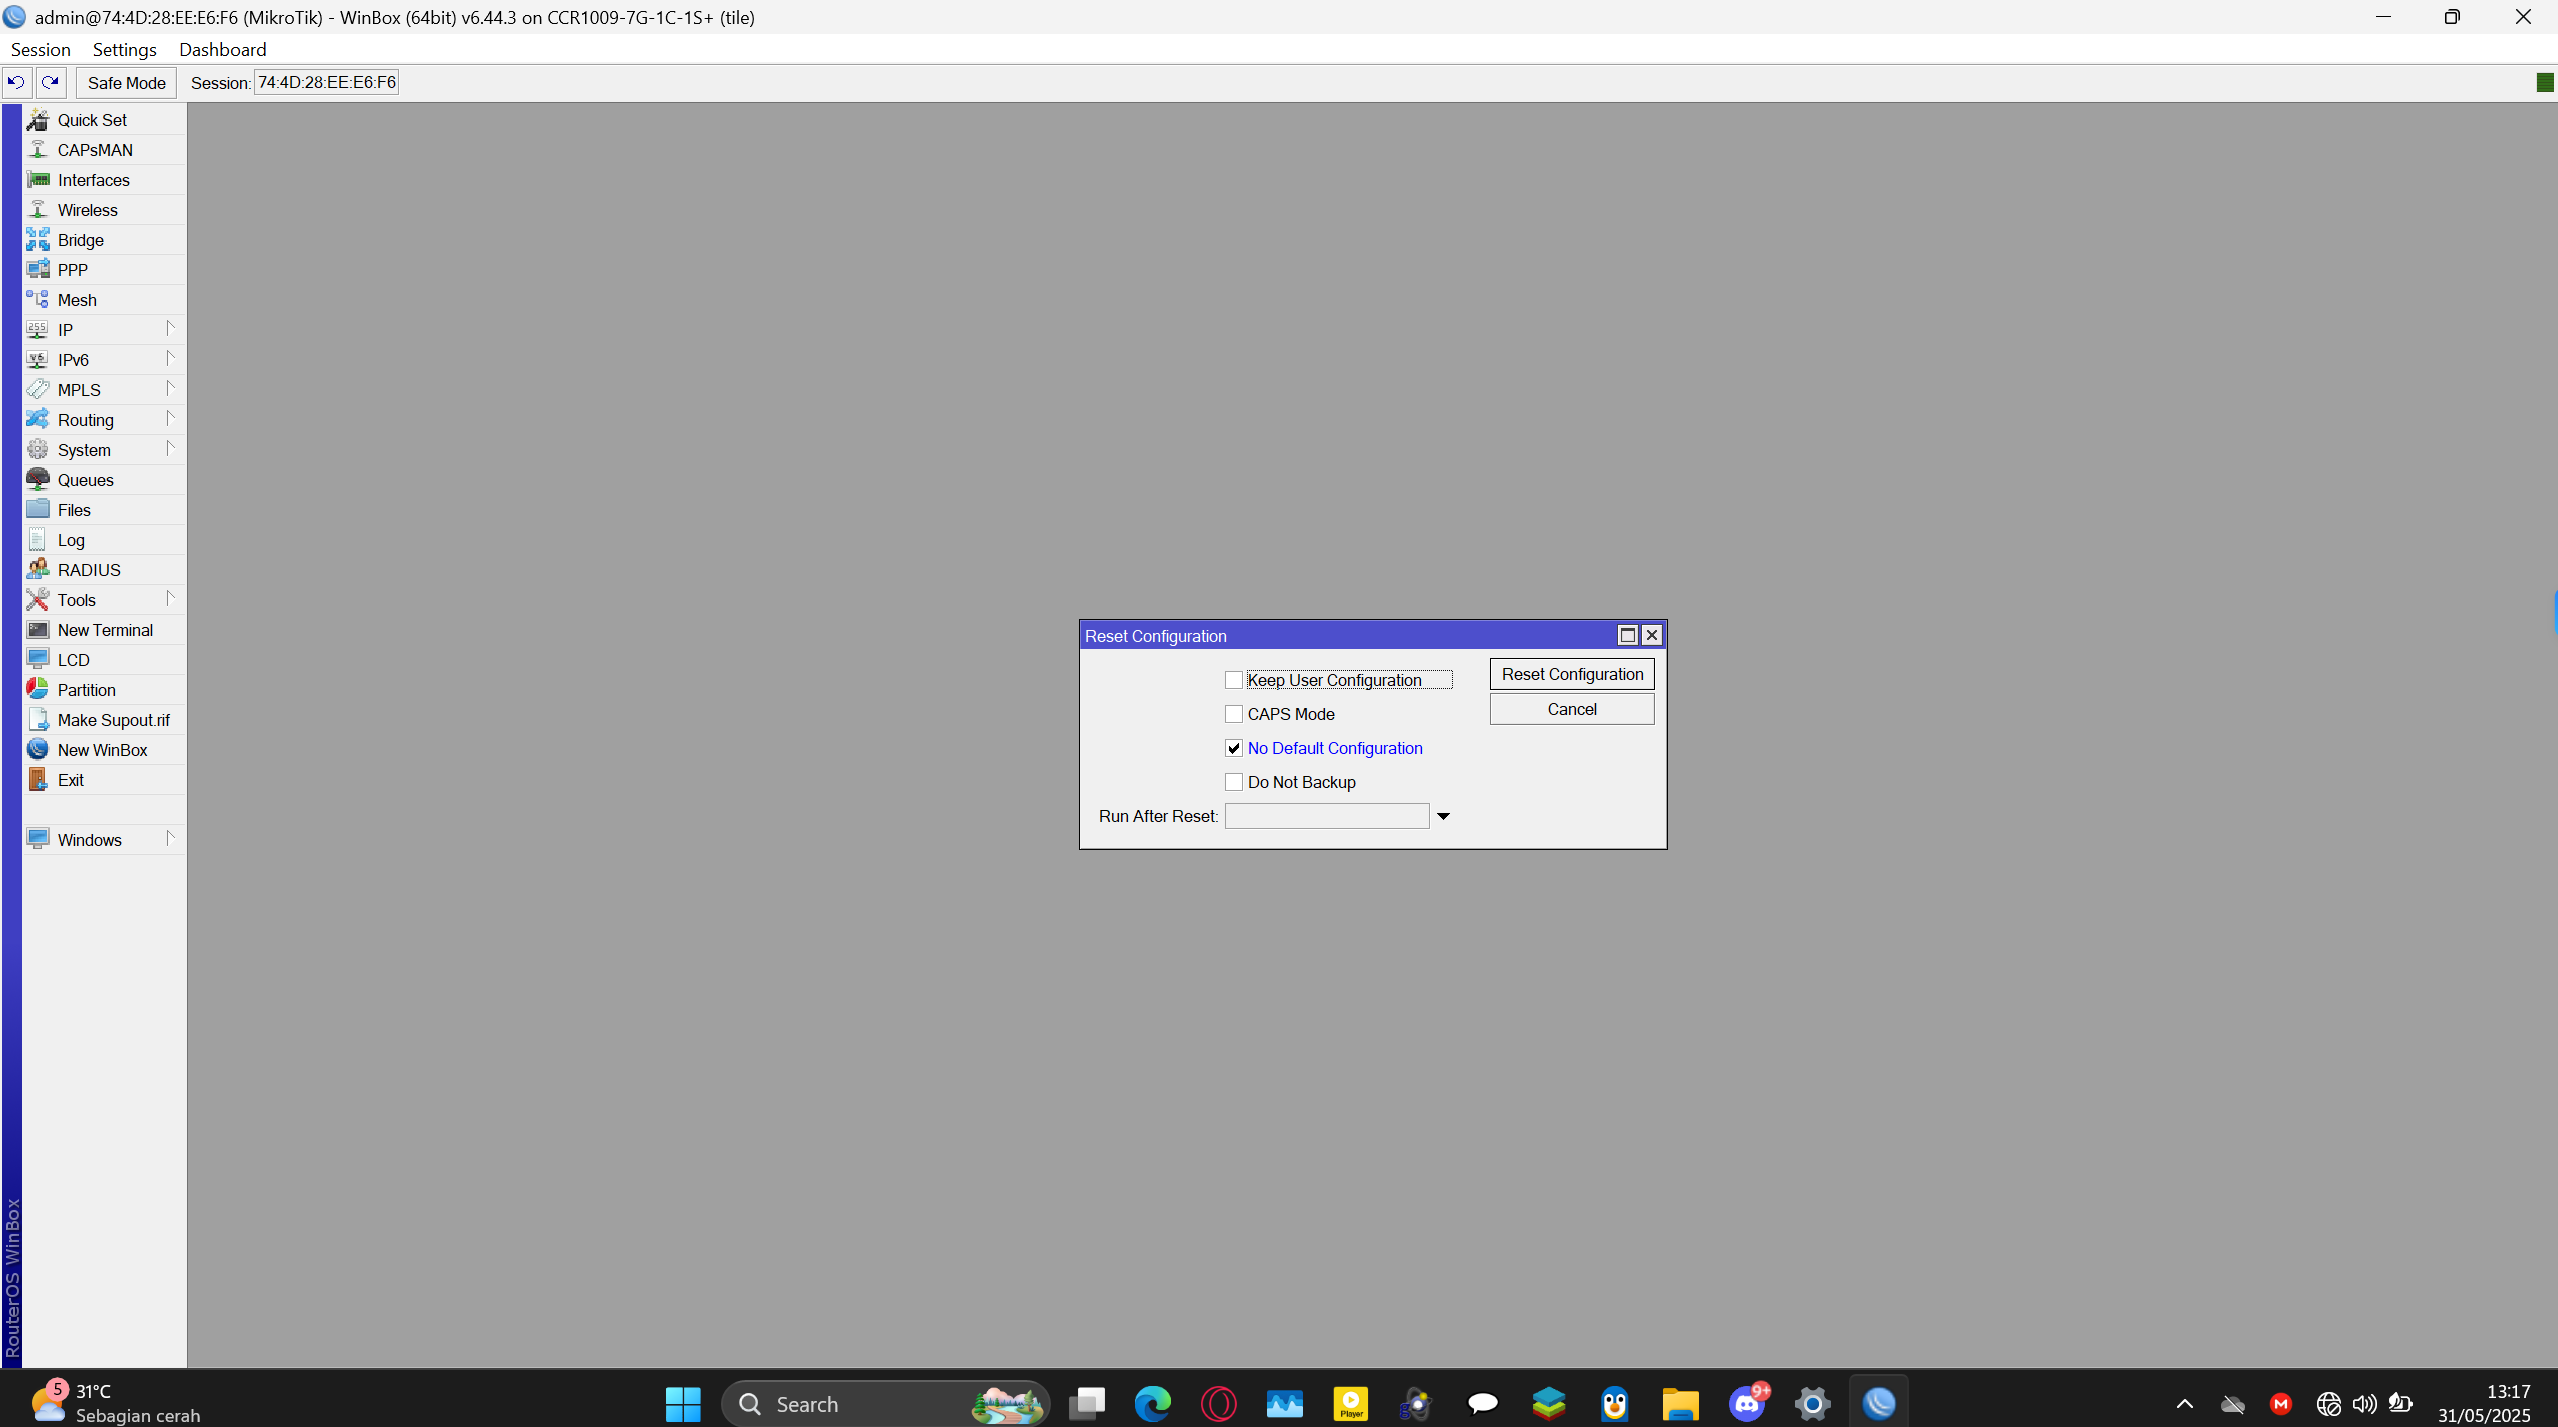
\includegraphics[width=0.5\linewidth]{P1/img/2.png}
        \caption{Reset Configuration}
        \label{fig:gambar4}
    \end{figure}
    \item Lakukan konfigurasi DCHP client pada router A terhadap ether 1
     \begin{figure}[H]
        \centering
        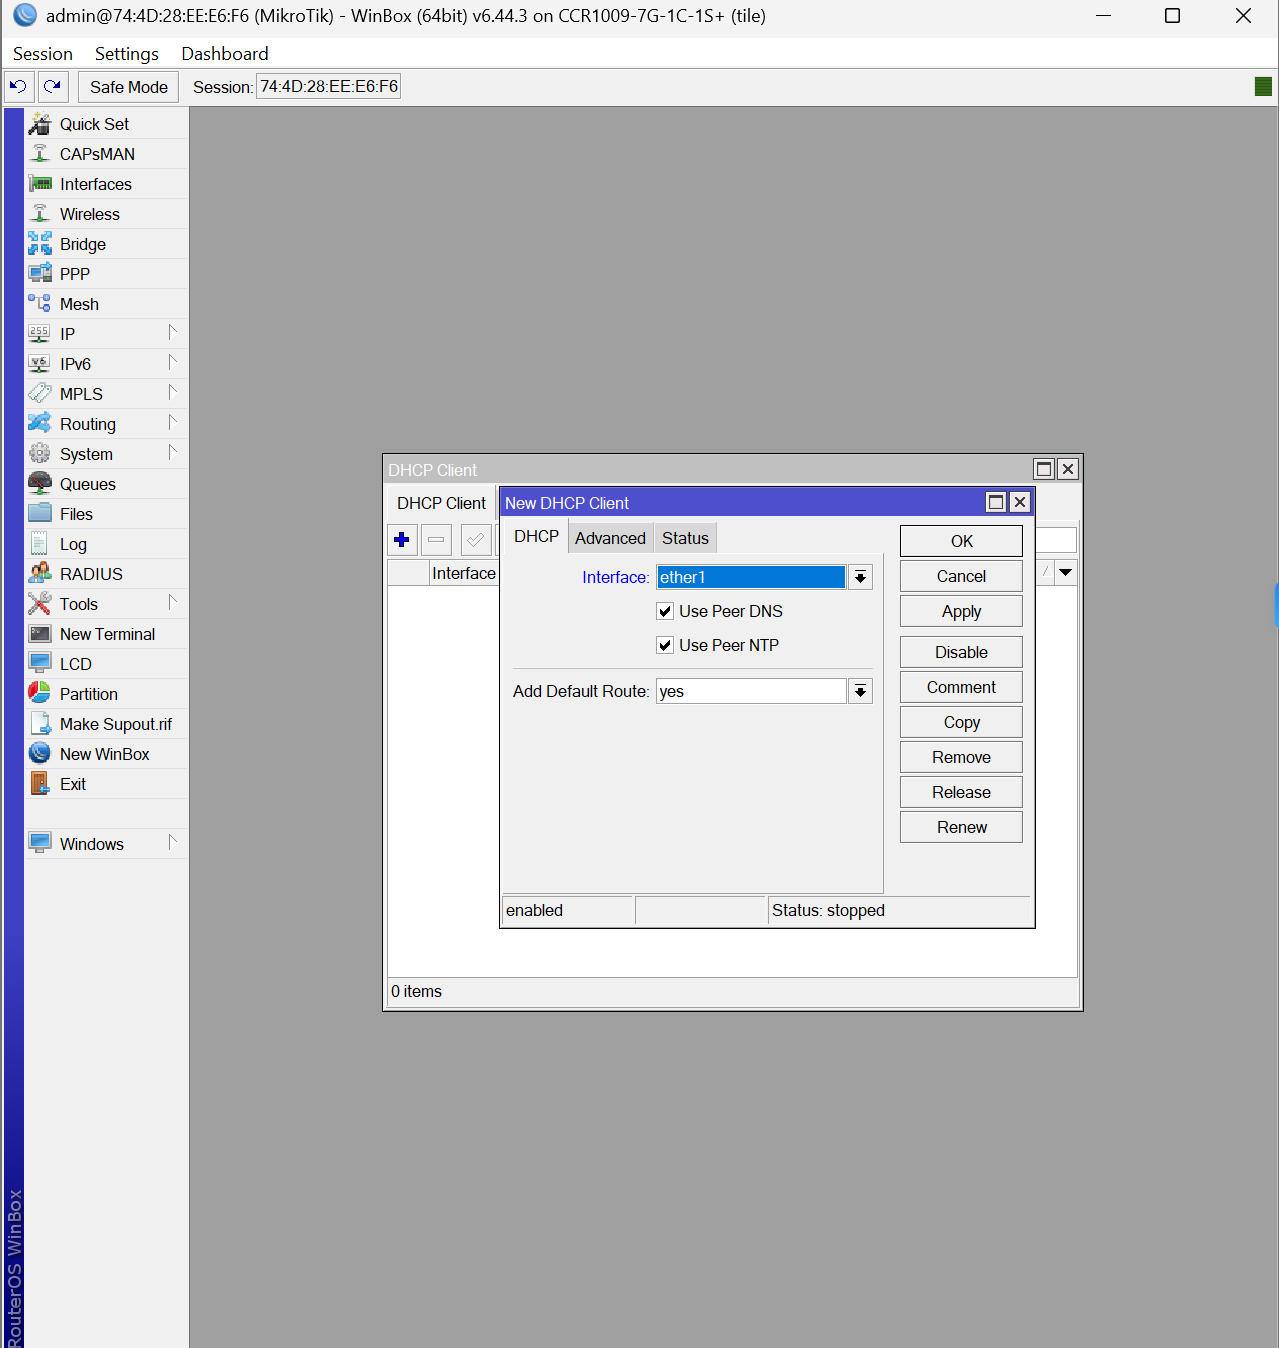
\includegraphics[width=0.5\linewidth]{P1/img/3.png}
        \caption{Atur DCHPnya}
        \label{fig:gambar4}
    \end{figure}
    \item Tambahkan alamat IP ether 1
     \begin{figure}[H]
        \centering
        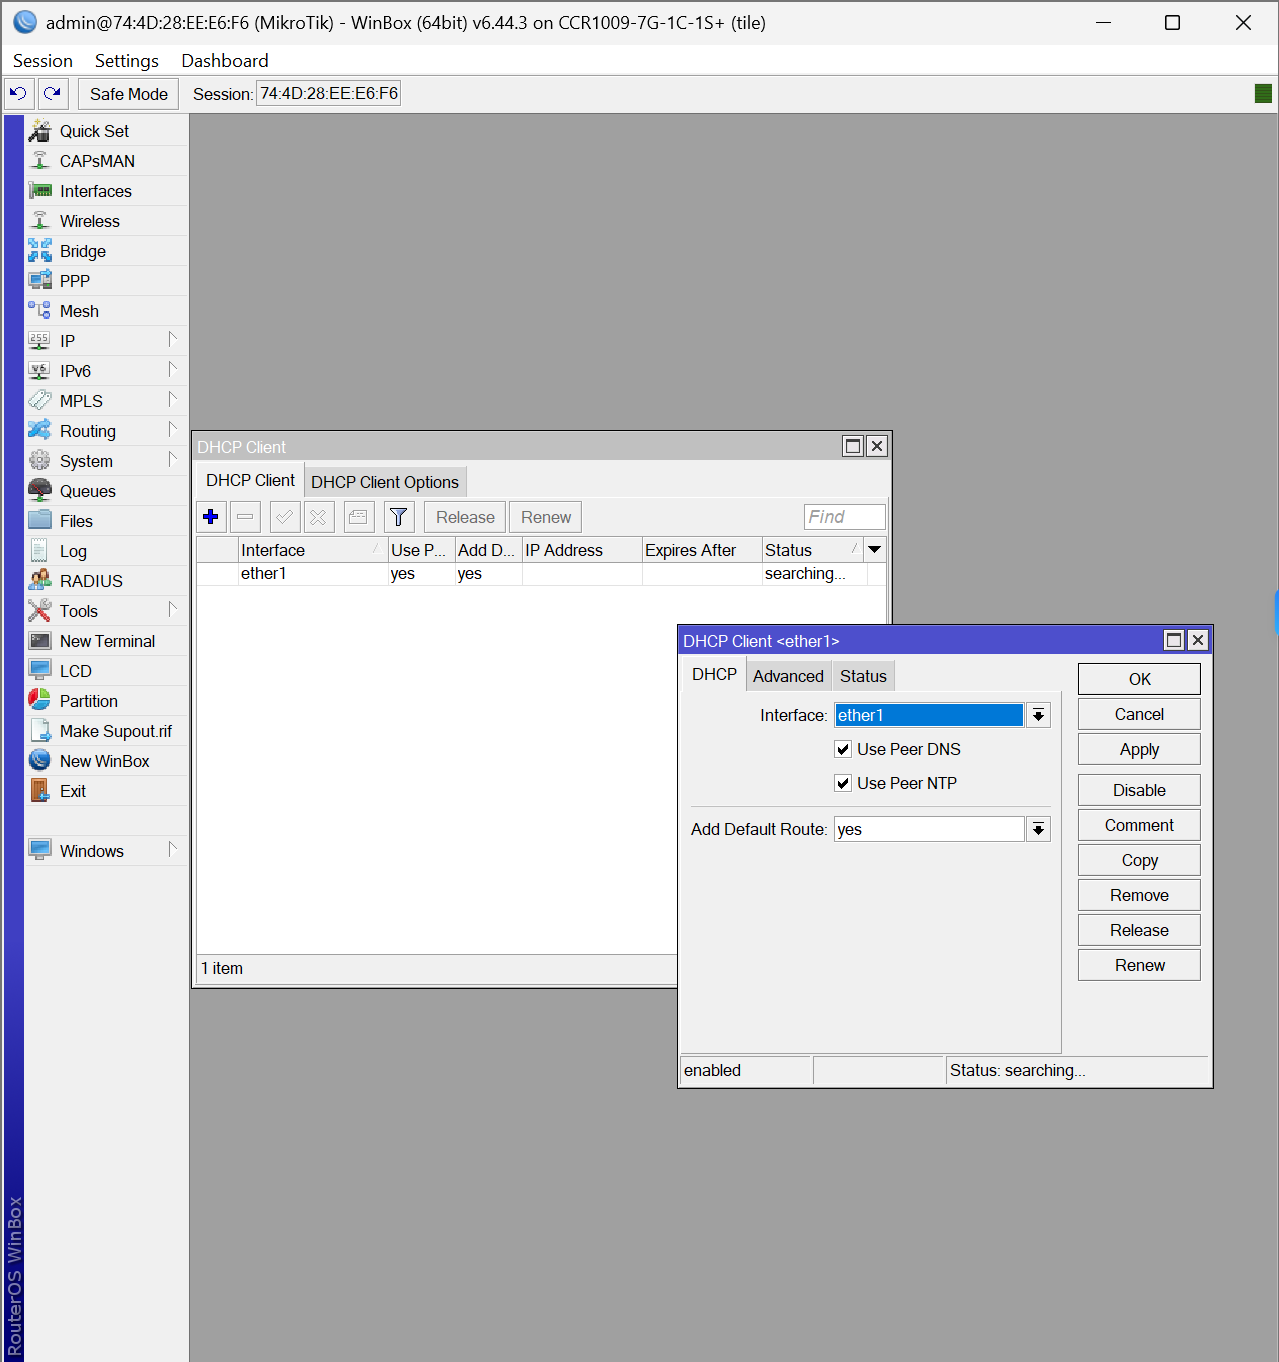
\includegraphics[width=0.5\linewidth]{P1/img/4.png}
        \caption{Atur alamat IPnya}
        \label{fig:gambar4}
    \end{figure}
    \item Konfigurasi DCHP server-nya
     \begin{figure}[H]
        \centering
        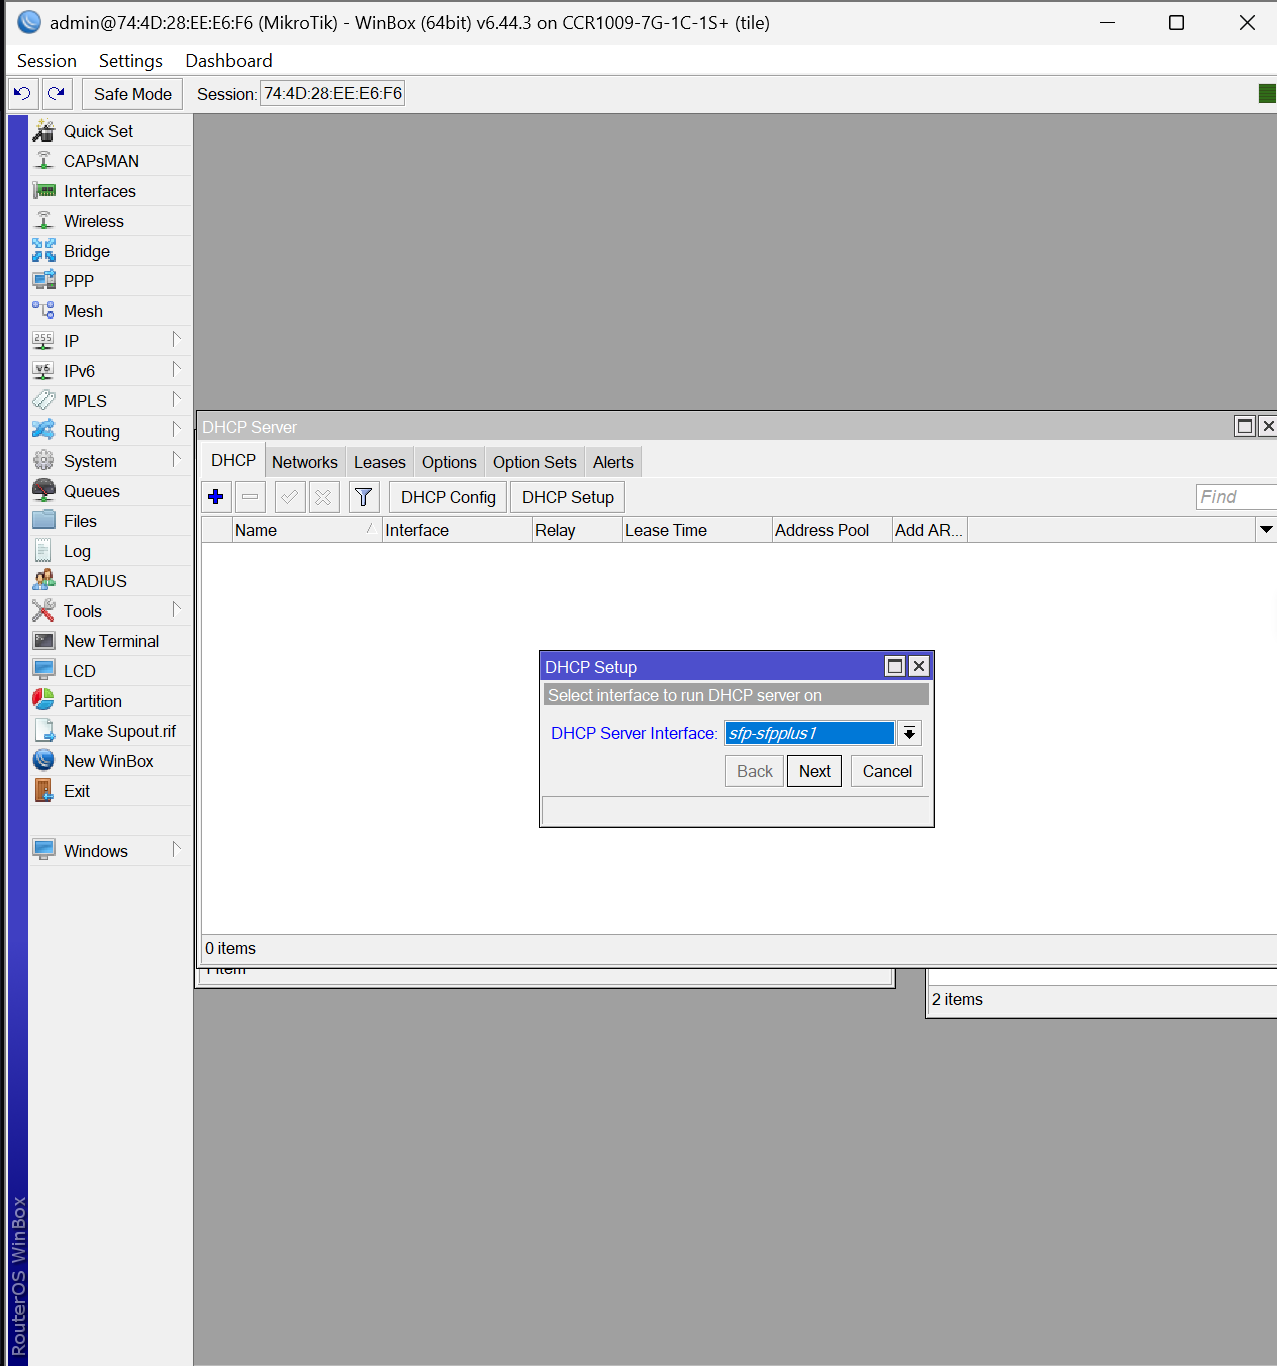
\includegraphics[width=0.5\linewidth]{P1/img/6.png}
        \caption{Atur DCHPnya}
        \label{fig:gambar4}
    \end{figure}
    \item Setelah itu, konfigurasikan Network Address Translation (NAT)
     \begin{figure}[H]
        \centering
        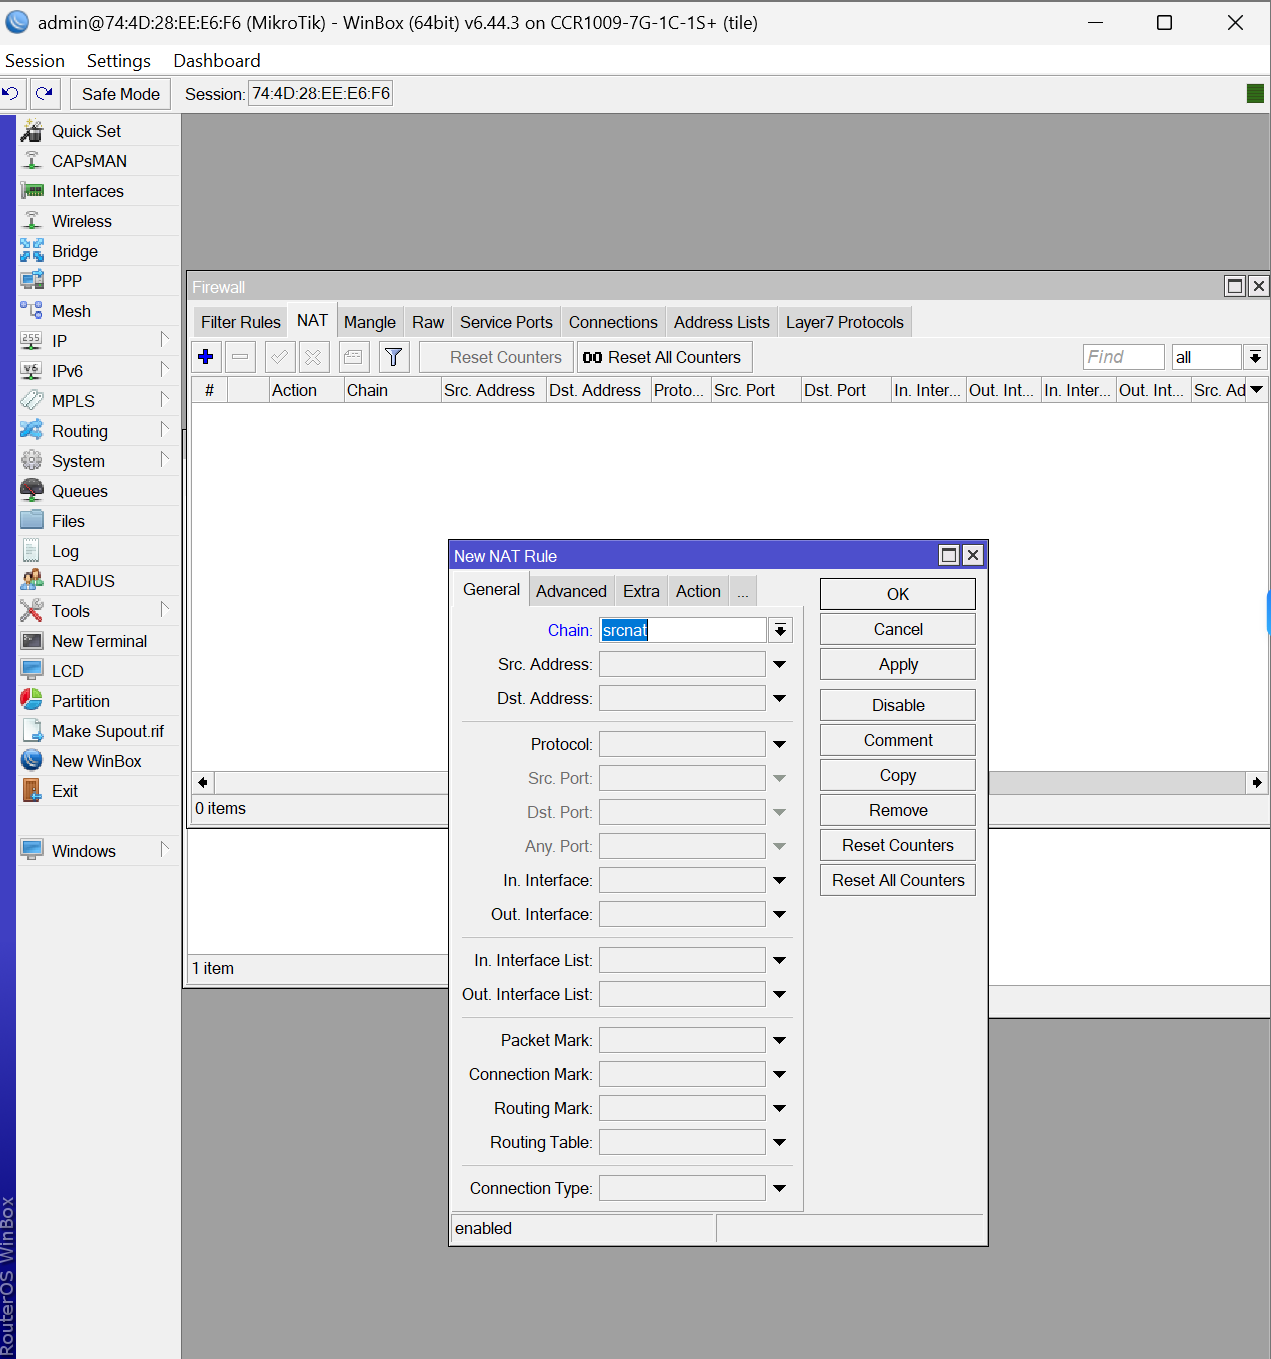
\includegraphics[width=0.5\linewidth]{P1/img/8.png}
        \caption{Pengaturan di Tab Generalnya}
        \label{fig:gambar4}
    \end{figure}
    \begin{figure}[H]
        \centering
        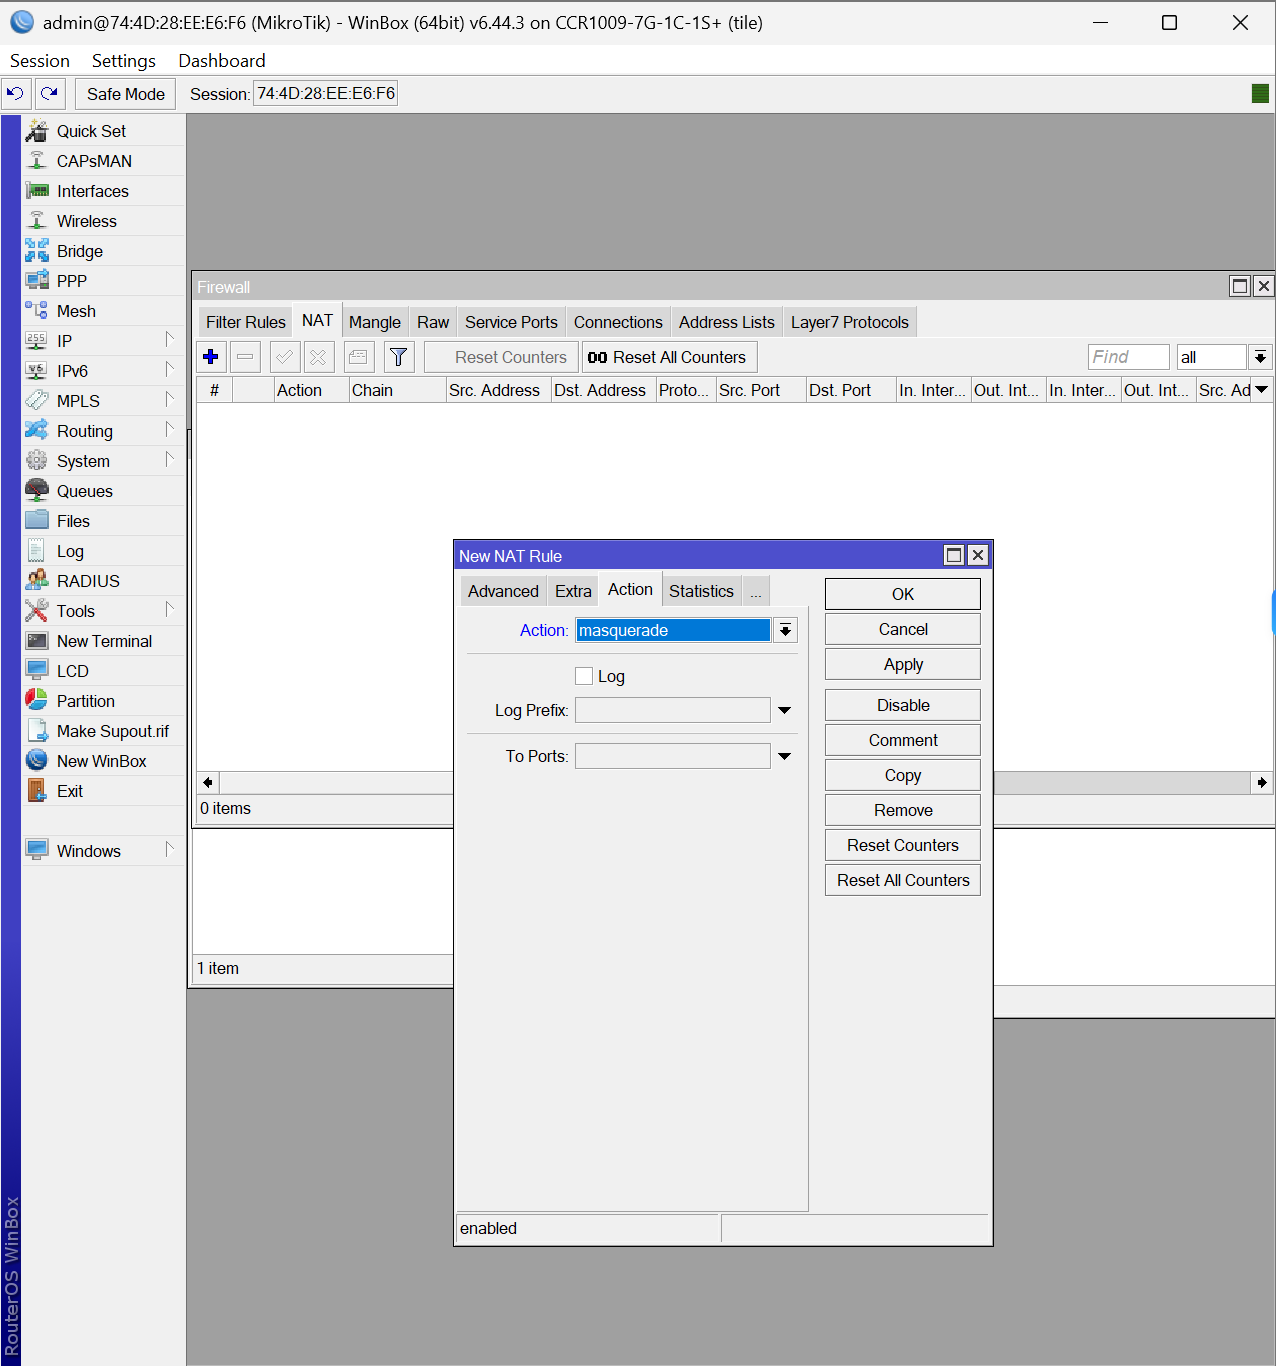
\includegraphics[width=0.5\linewidth]{P1/img/9.png}
        \caption{Pengaturan di Tab Actionnya}
        \label{fig:gambar4}
    \end{figure}
    \item Sekarang konfigurasikan firewallnya.
     \begin{figure}[H]
        \centering
        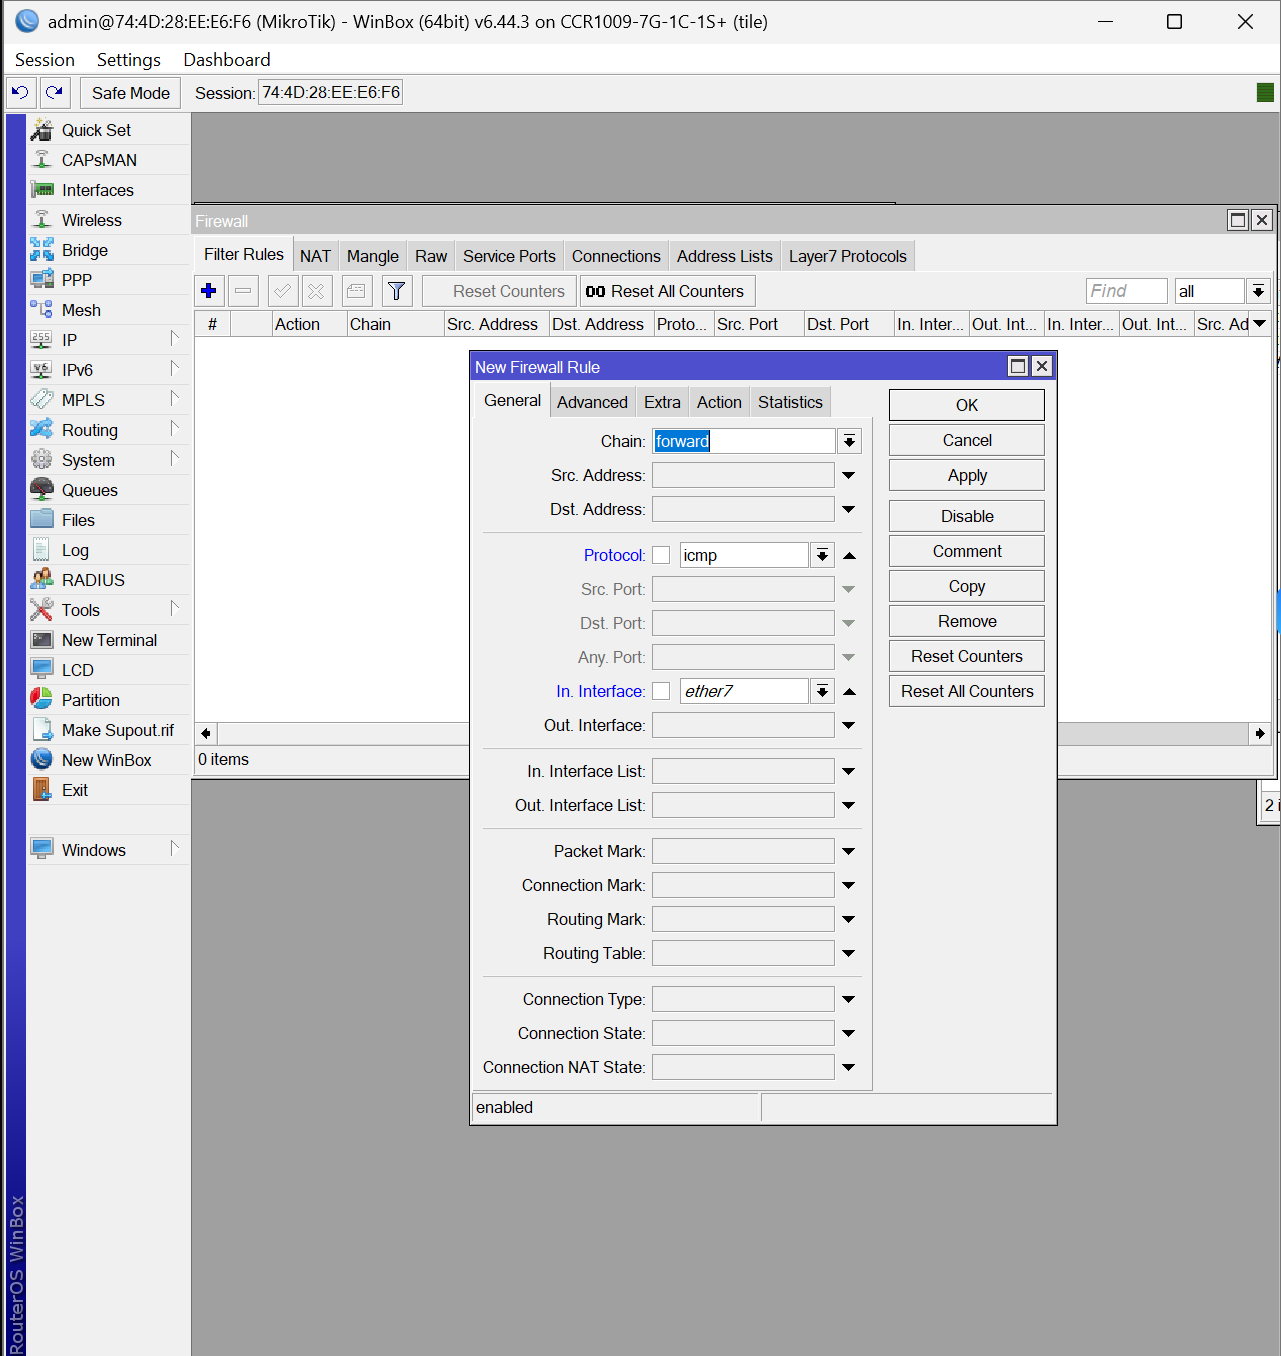
\includegraphics[width=0.5\linewidth]{P1/img/14.png}
        \caption{Pengaturan Firewall}
        \label{fig:gambar4}
    \end{figure}
     \begin{figure}[H]
        \centering
        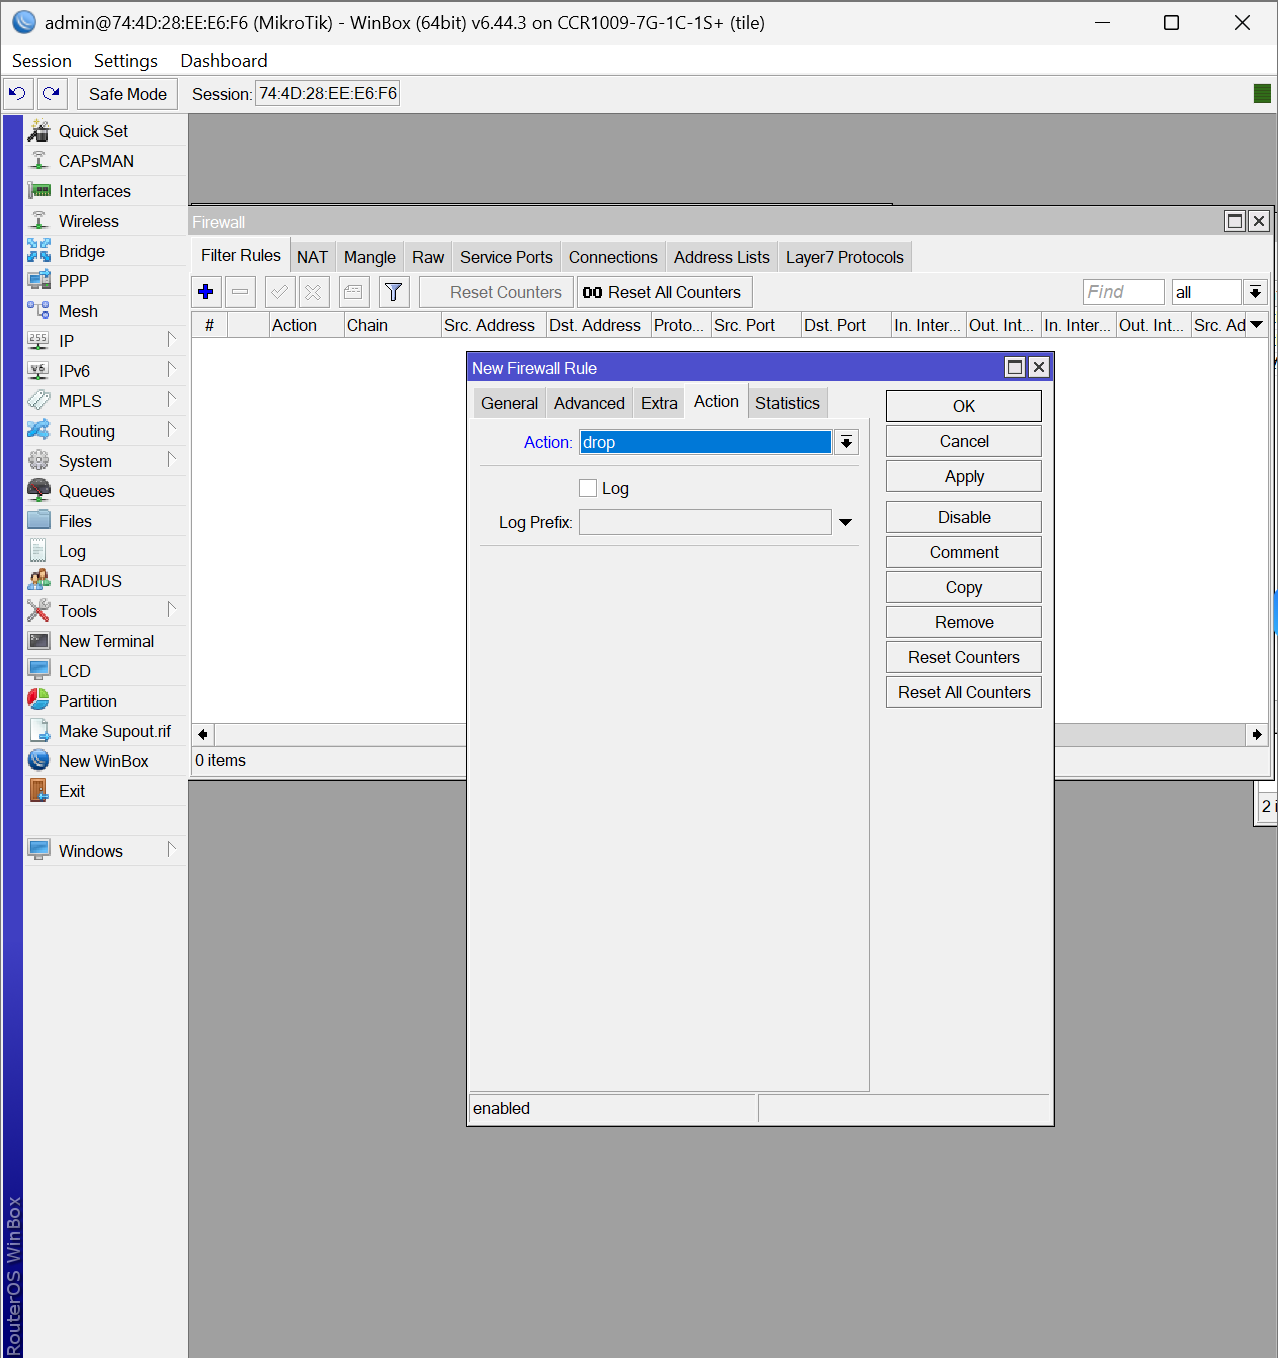
\includegraphics[width=0.5\linewidth]{P1/img/15.png}
        \caption{Pengaturan Firewall}
        \label{fig:gambar4}
    \end{figure}
     \begin{figure}[H]
        \centering
        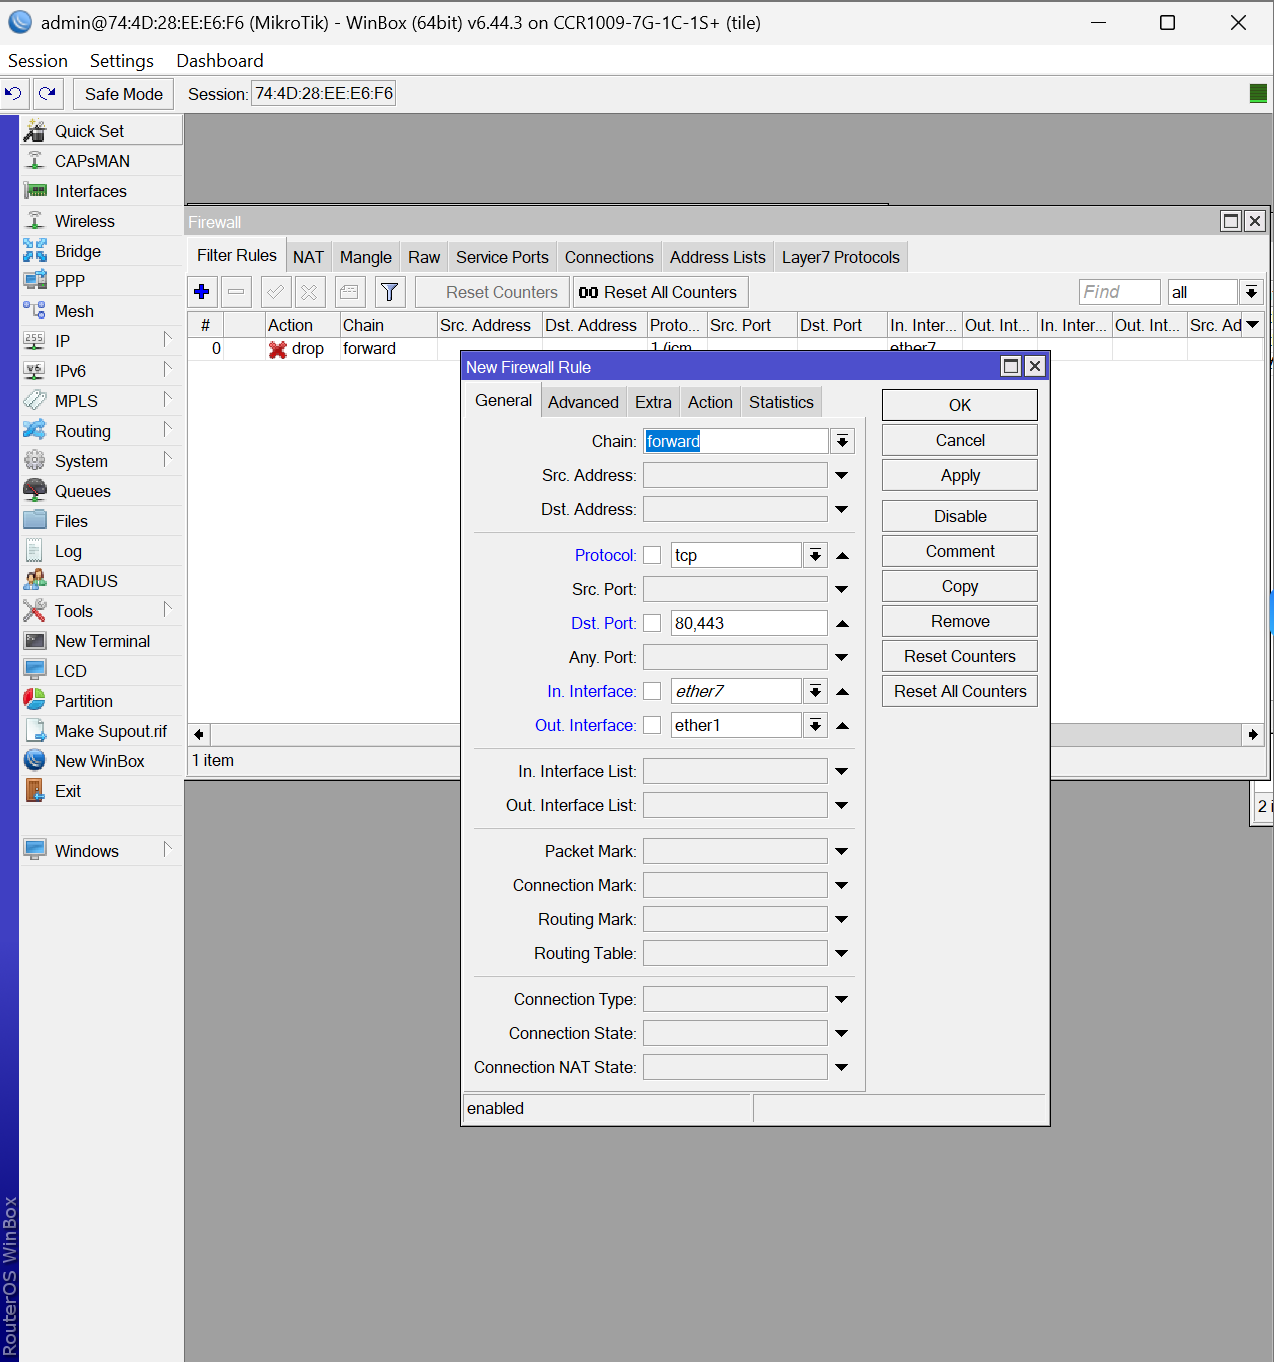
\includegraphics[width=0.5\linewidth]{P1/img/16.png}
        \caption{Pengaturan Firewall}
        \label{fig:gambar4}
    \end{figure}
     \begin{figure}[H]
        \centering
        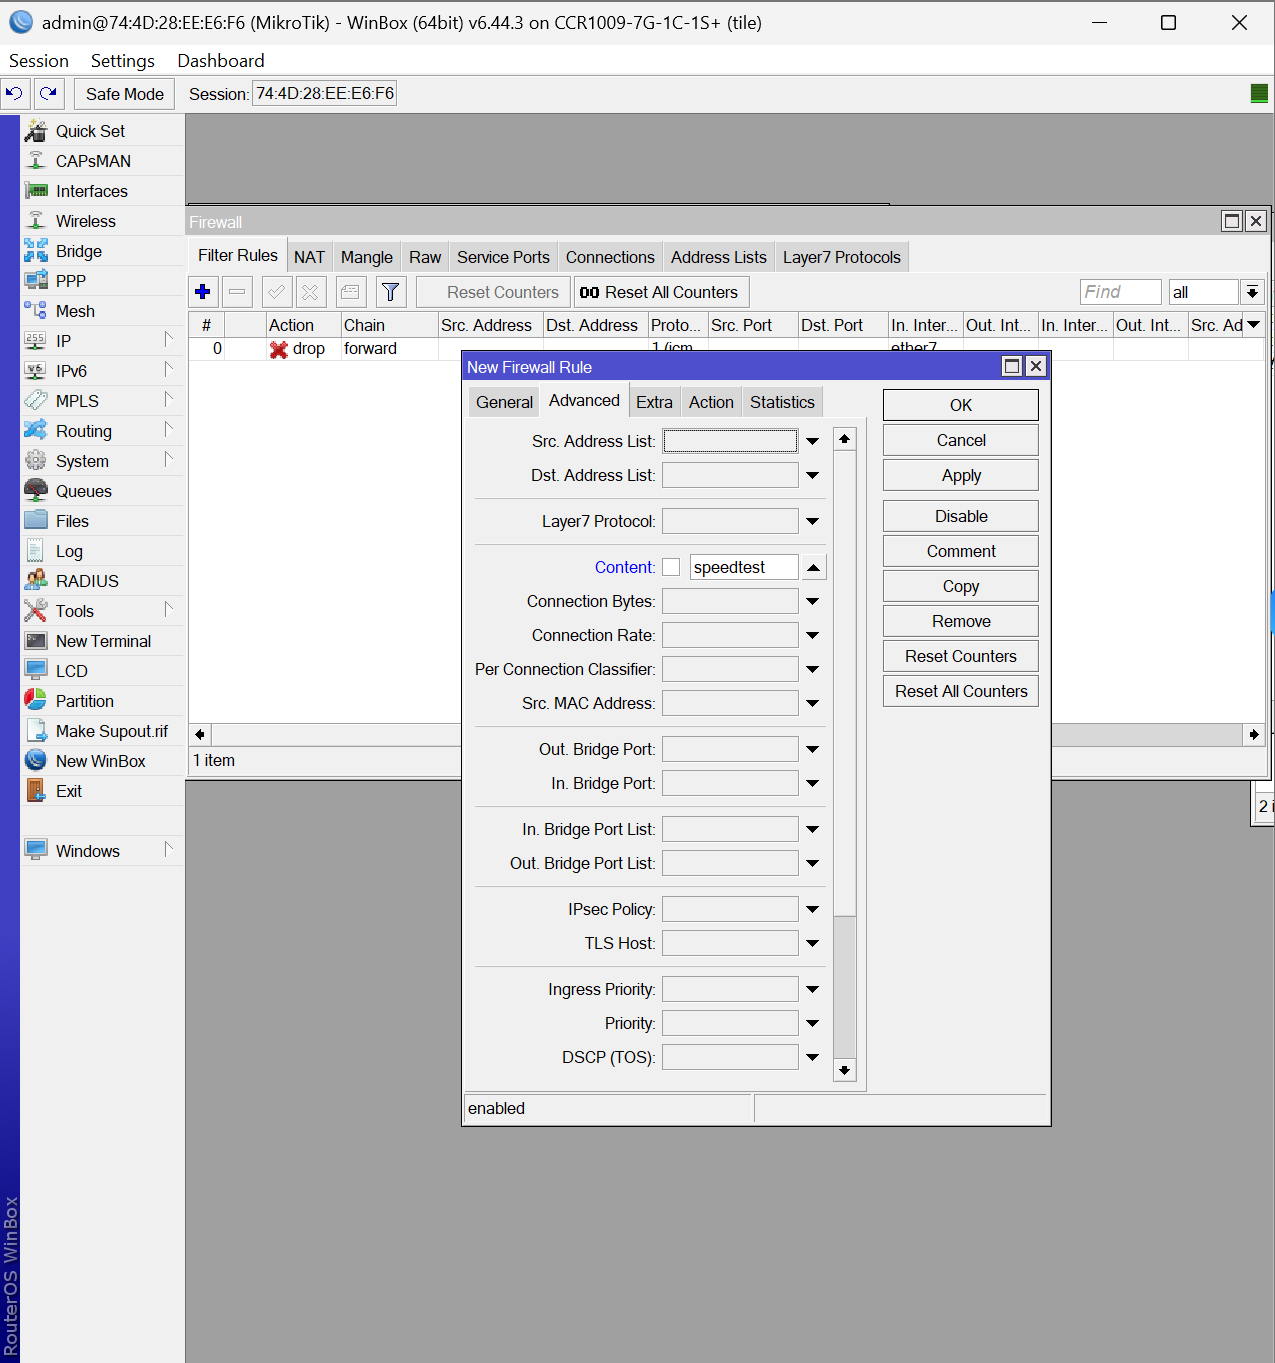
\includegraphics[width=0.5\linewidth]{P1/img/17.png}
        \caption{Pengaturan Firewall}
        \label{fig:gambar4}
    \end{figure}
     \begin{figure}[H]
        \centering
        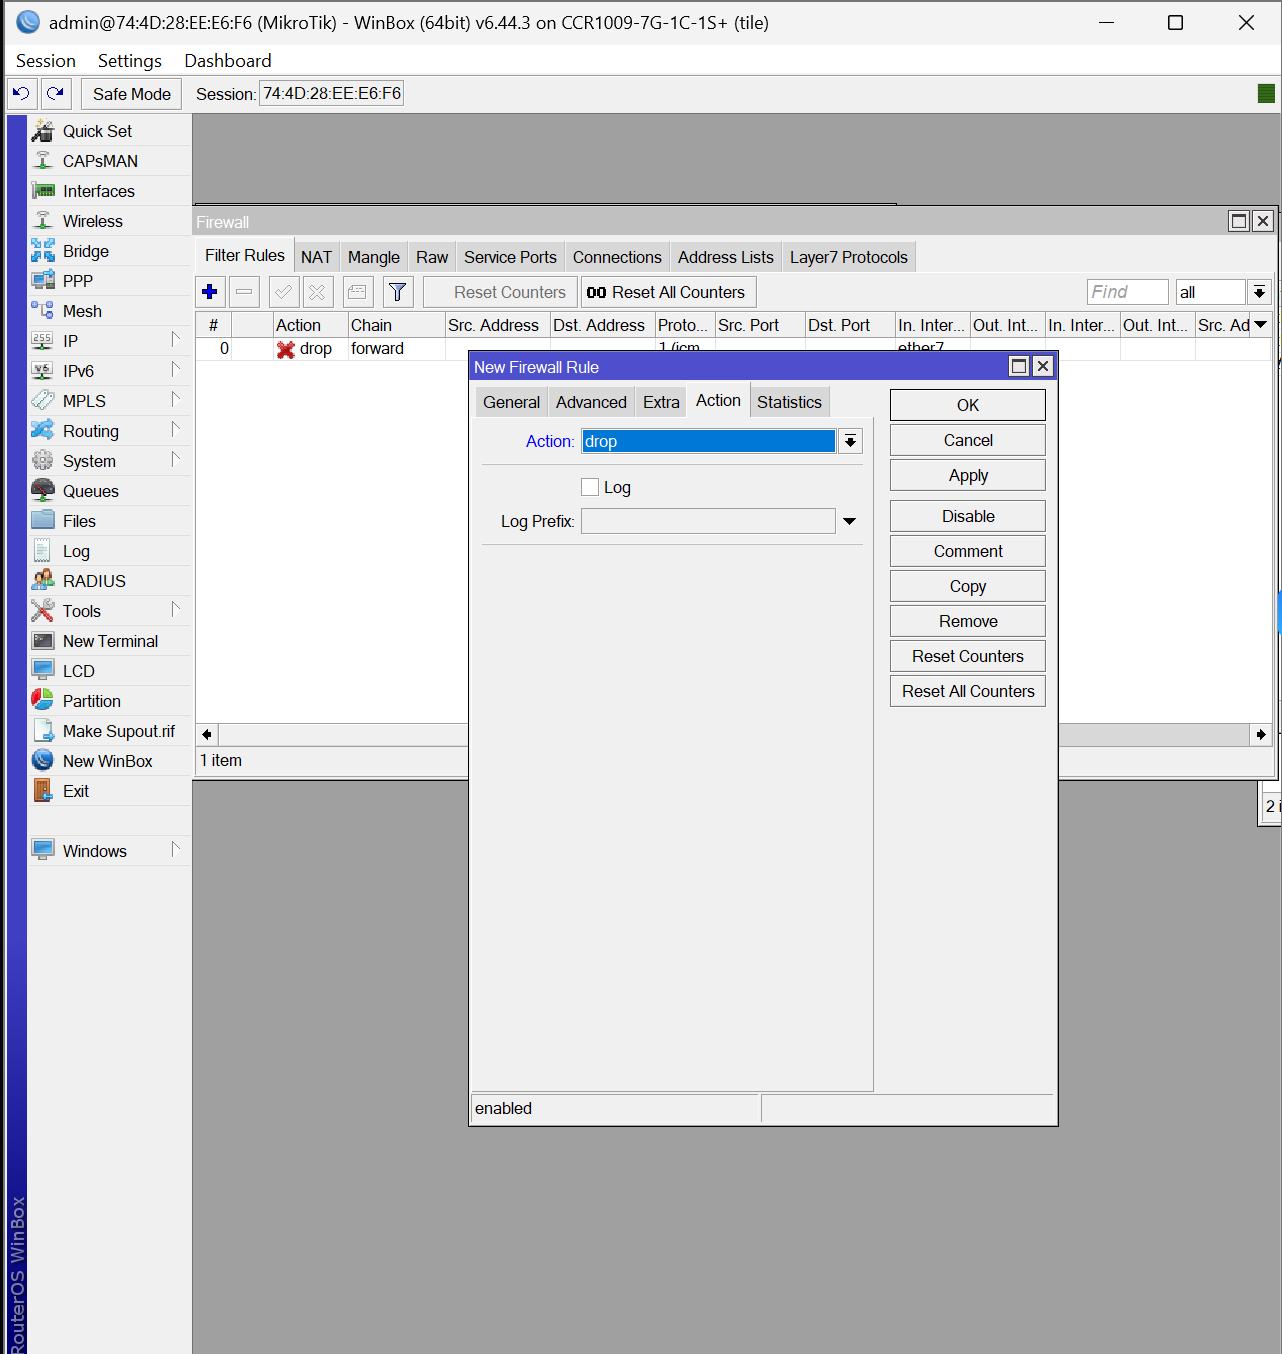
\includegraphics[width=0.5\linewidth]{P1/img/18.png}
        \caption{Pengaturan Firewall}
        \label{fig:gambar4}
    \end{figure}
    \item Konfigurasikan Bridge pada router B
     \begin{figure}[H]
        \centering
        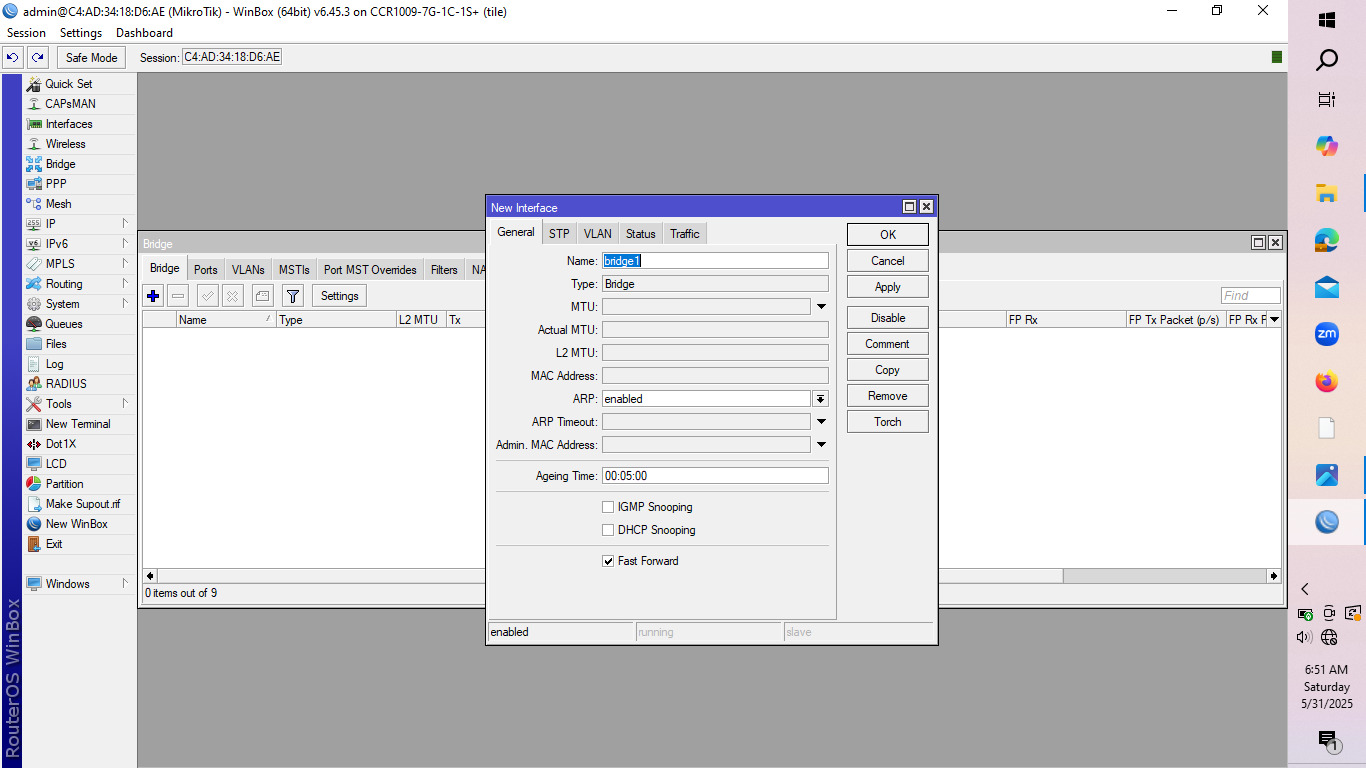
\includegraphics[width=0.5\linewidth]{P1/img/22.jpeg}
        \caption{Pengaturan Bridge}
        \label{fig:gambar4}
    \end{figure}
     \begin{figure}[H]
        \centering
        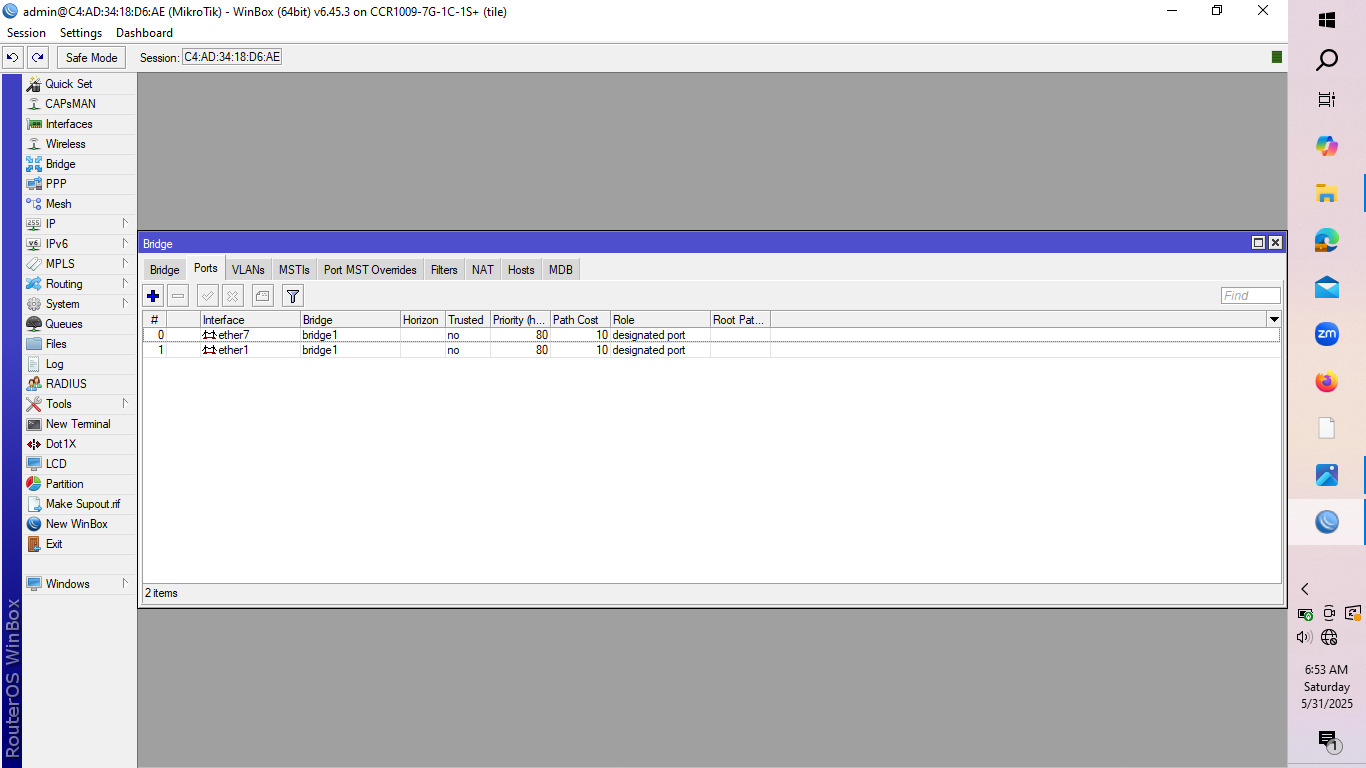
\includegraphics[width=0.5\linewidth]{P1/img/21.jpeg}
        \caption{Pengaturan Bridge}
        \label{fig:gambar4}
    \end{figure}
    \item Liat alamat IP pada laptop menggunakan CMD
     \begin{figure}[H]
        \centering
        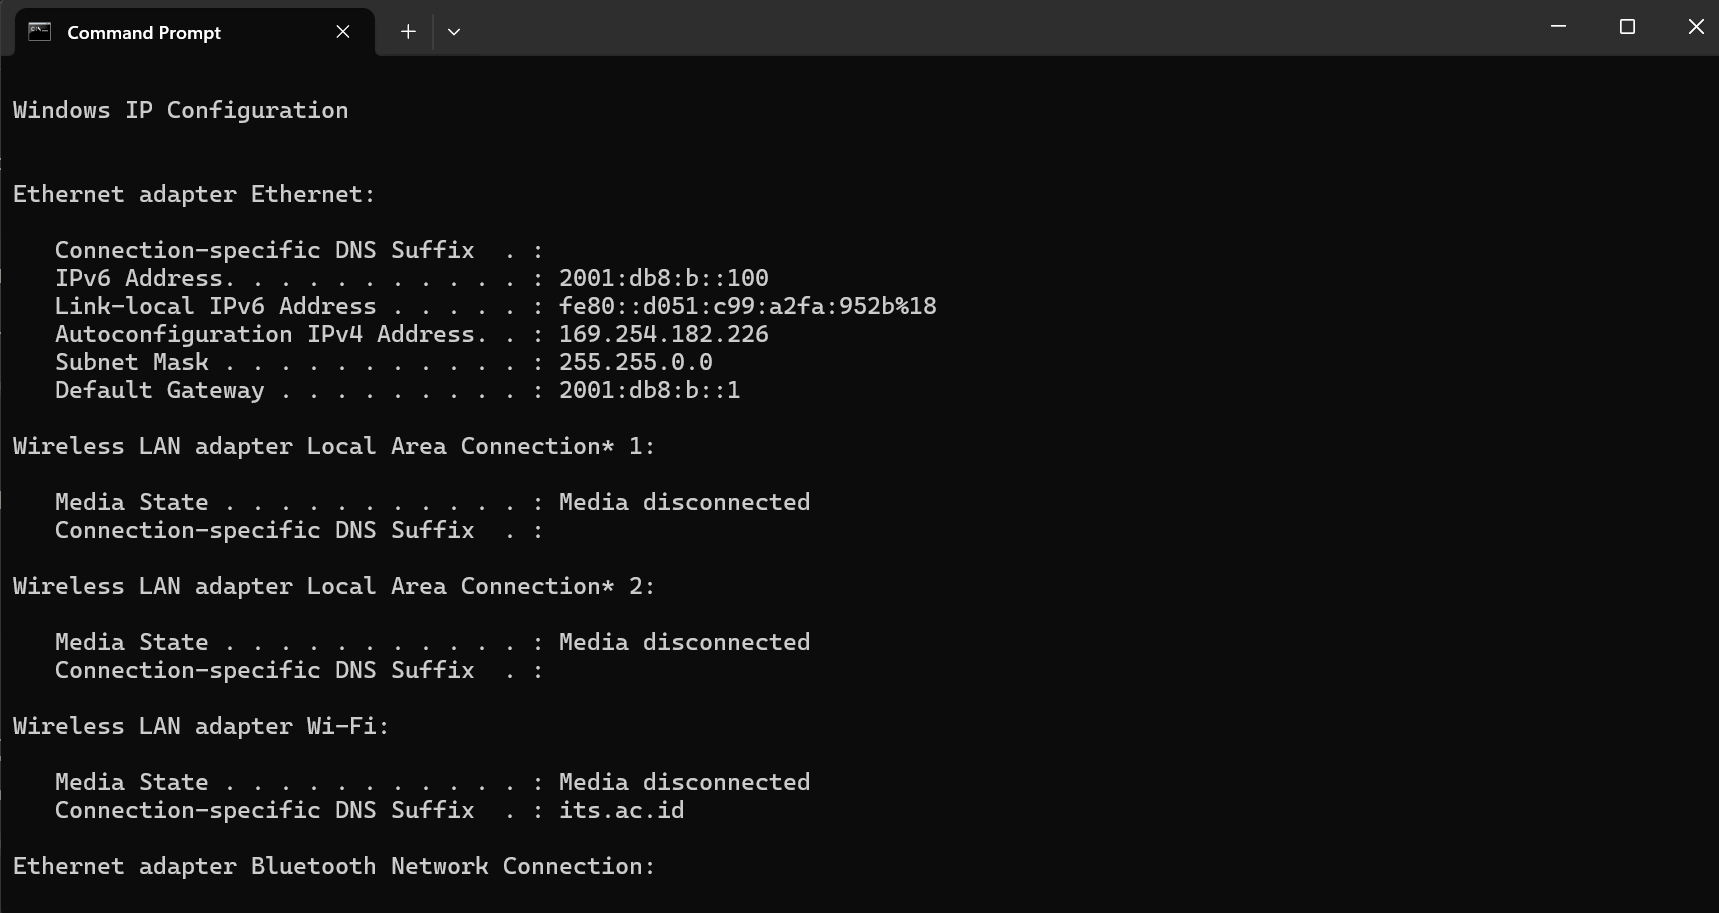
\includegraphics[width=0.5\linewidth]{P1/img/19.png}
        \caption{Catat IP addressnya}
        \label{fig:gambar4}
    \end{figure}
    \item Uji Coba Konfigurasinya
     \begin{figure}[H]
        \centering
        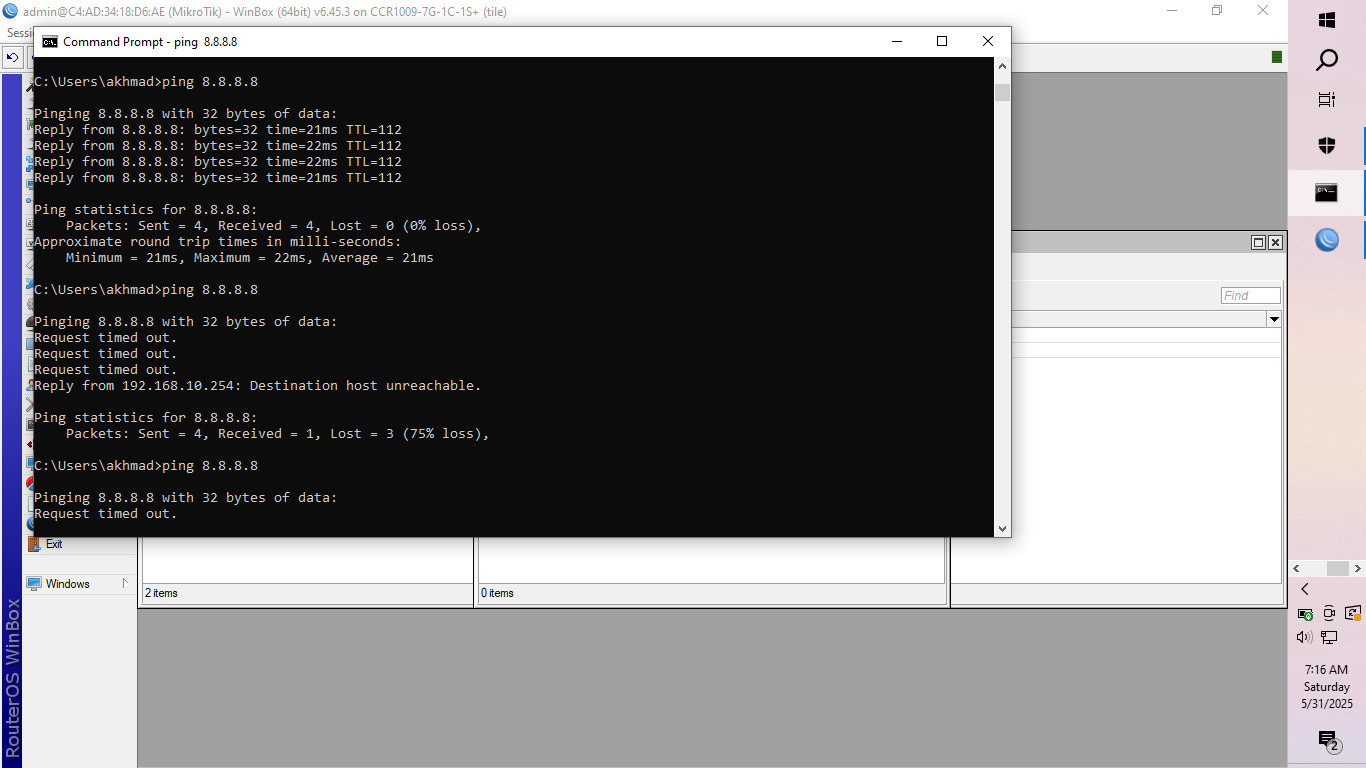
\includegraphics[width=0.5\linewidth]{P1/img/23.jpeg}
        \caption{Uji Konfigurasi}
        \label{fig:gambar4}
    \end{figure}

\end{enumerate}


\section{Analisis Hasil Percobaan}

Pada praktikum ini dilakukan konfigurasi fitur keamanan dan translasi alamat jaringan menggunakan perangkat MikroTik, yaitu Firewall dan NAT (Network Address Translation). Praktikum ini bertujuan untuk memahami bagaimana mekanisme pengaturan lalu lintas data dan penerjemahan alamat IP bekerja dalam jaringan, serta dampaknya terhadap konektivitas dan keamanan. Dua router digunakan dalam skenario ini, dengan Router A sebagai pengakses internet melalui DHCP Client dan NAT, sementara Router B dikonfigurasi sebagai bridge agar laptop klien dapat terkoneksi melalui jaringan internal.
\\
Langkah awal dilakukan dengan mereset konfigurasi router agar tidak terjadi konflik pengaturan. Router A kemudian disambungkan ke internet melalui ether1 dan dikonfigurasi sebagai DHCP client. IP statis ditambahkan ke ether7 untuk membangun koneksi lokal dengan switch. Router A juga dikonfigurasi sebagai DHCP server yang mendistribusikan alamat IP ke klien melalui ether7. Dengan konfigurasi ini, perangkat klien dapat memperoleh IP secara otomatis, mempermudah integrasi perangkat baru ke jaringan.
\\
Selanjutnya dilakukan konfigurasi NAT dengan menetapkan aturan `src-nat` dan aksi `masquerade`, yang memungkinkan perangkat dalam jaringan internal untuk mengakses internet menggunakan satu IP publik. Pengujian dilakukan dengan perintah ping ke 8.8.8.8, dan hasil menunjukkan koneksi berhasil dilakukan tanpa gangguan, menandakan NAT berfungsi dengan baik sebagai jembatan antara jaringan lokal dan internet.
\\
Untuk meningkatkan keamanan, firewall dikonfigurasi dengan dua jenis aturan: pemblokiran ICMP dan pemblokiran konten web. Aturan pemblokiran ICMP ditujukan untuk menolak lalu lintas ping dari klien di ether7, dan pengujian menunjukkan bahwa saat aturan aktif, ping ke internet akan menghasilkan respons "Request Timed Out". Setelah aturan dinonaktifkan, koneksi kembali normal. Ini membuktikan efektivitas firewall dalam mengontrol jenis lalu lintas tertentu.
\\
Aturan kedua adalah pemblokiran akses konten berdasarkan kata kunci "speedtest" pada trafik HTTP dan HTTPS. Saat diaktifkan, situs web seperti speedtest.net tidak dapat diakses oleh klien. Setelah aturan dinonaktifkan, situs dapat dibuka kembali dengan normal. Ini menunjukkan bahwa firewall mampu melakukan filter berdasarkan konten dan protokol, memberikan kontrol granular terhadap akses web.
\\
Router B dikonfigurasi sebagai bridge dengan menambahkan beberapa interface ke dalamnya, memungkinkan laptop terhubung melalui port yang sama ke jaringan lokal. Konfigurasi IP pada laptop disetel ke DHCP, dan verifikasi melalui perintah `ipconfig` menunjukkan bahwa alamat IP berhasil diperoleh dari DHCP server Router A. Ini menandakan bahwa bridge dan distribusi IP berjalan dengan baik.


\section{Hasil Tugas Modul}
\begin{enumerate}
\item Buatlah topologi sederhana di Cisco Packet Tracer dengan:
1 Router
1 Switch
3 PC (LAN)
1 Server (Internet/Public)
    \begin{figure}[H]
        \centering
        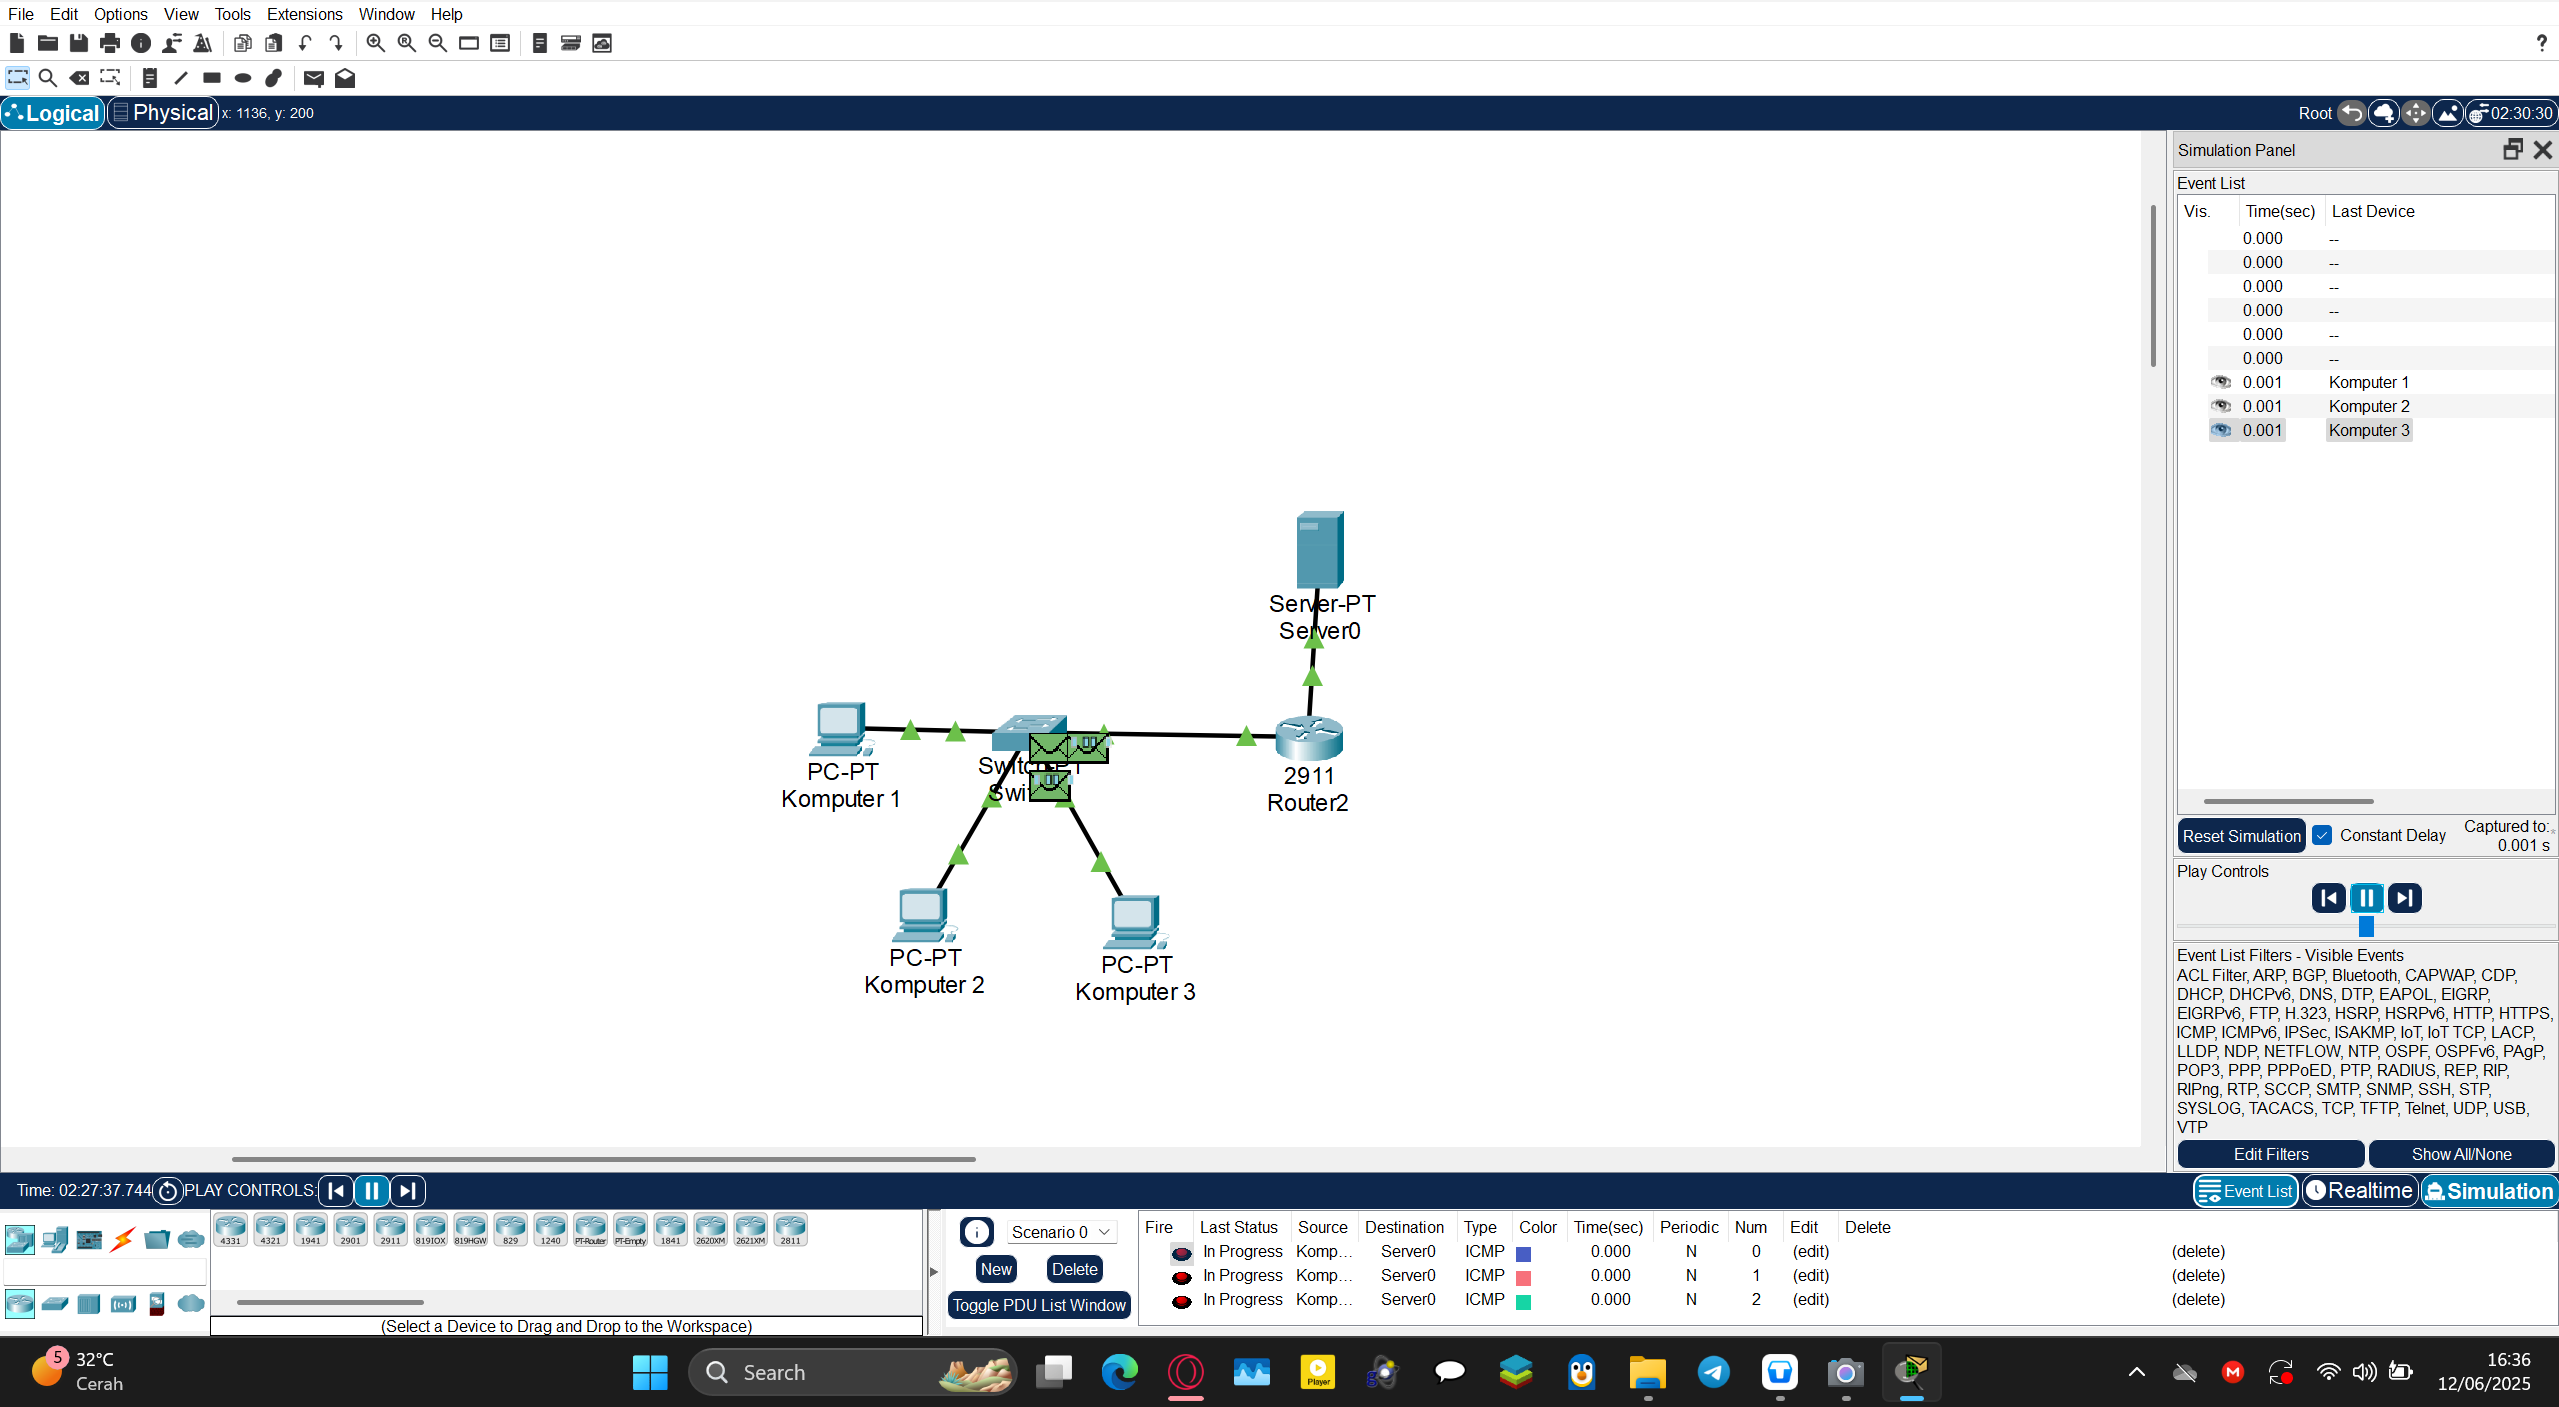
\includegraphics[width=0.8\linewidth]{P1/img/24.png}
        \caption{Hasil dari cisco packet tracer}
        \label{fig:gambar4}
    \end{figure}
\item Konfigurasi NAT: Buat agar semua PC bisa mengakses Server menggunakan IP publik Router.
  \begin{figure}[H]
        \centering
        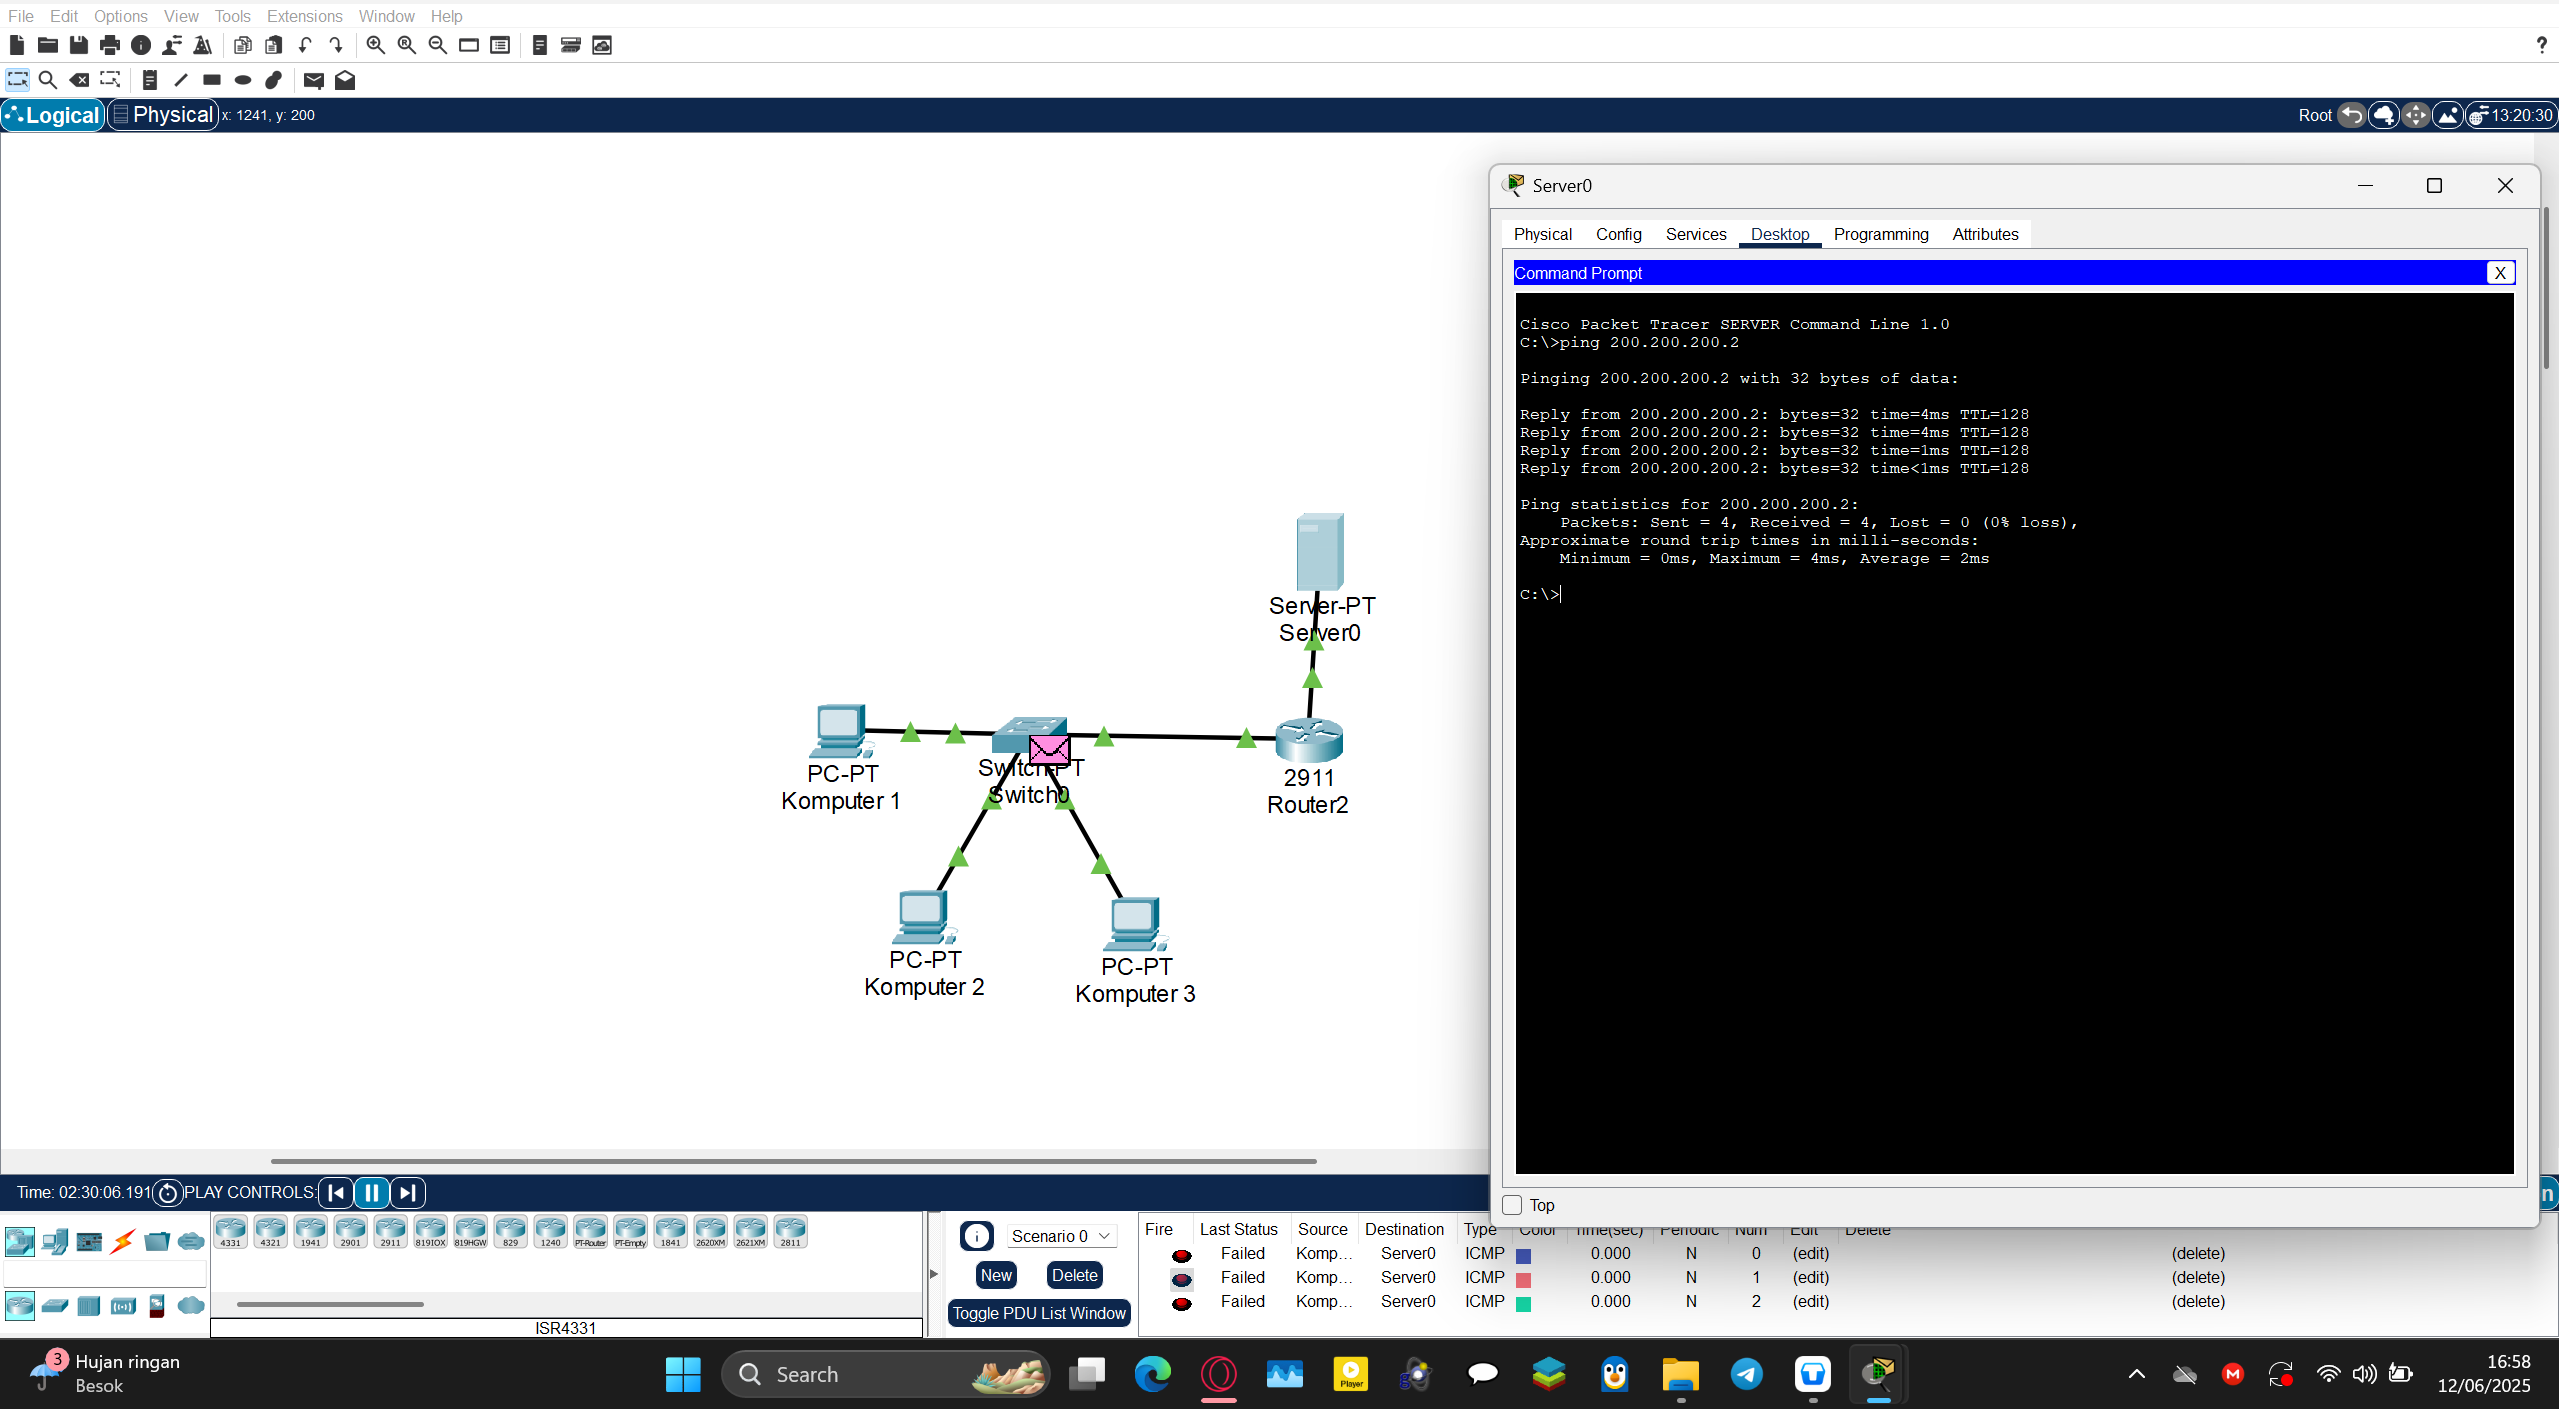
\includegraphics[width=0.8\linewidth]{P1/img/25.png}
        \caption{Hasil konfigurasi}
        \label{fig:gambar4}
    \end{figure}
\item Konfigurasi Firewall (ACL):
\begin{figure}[H]
        \centering
        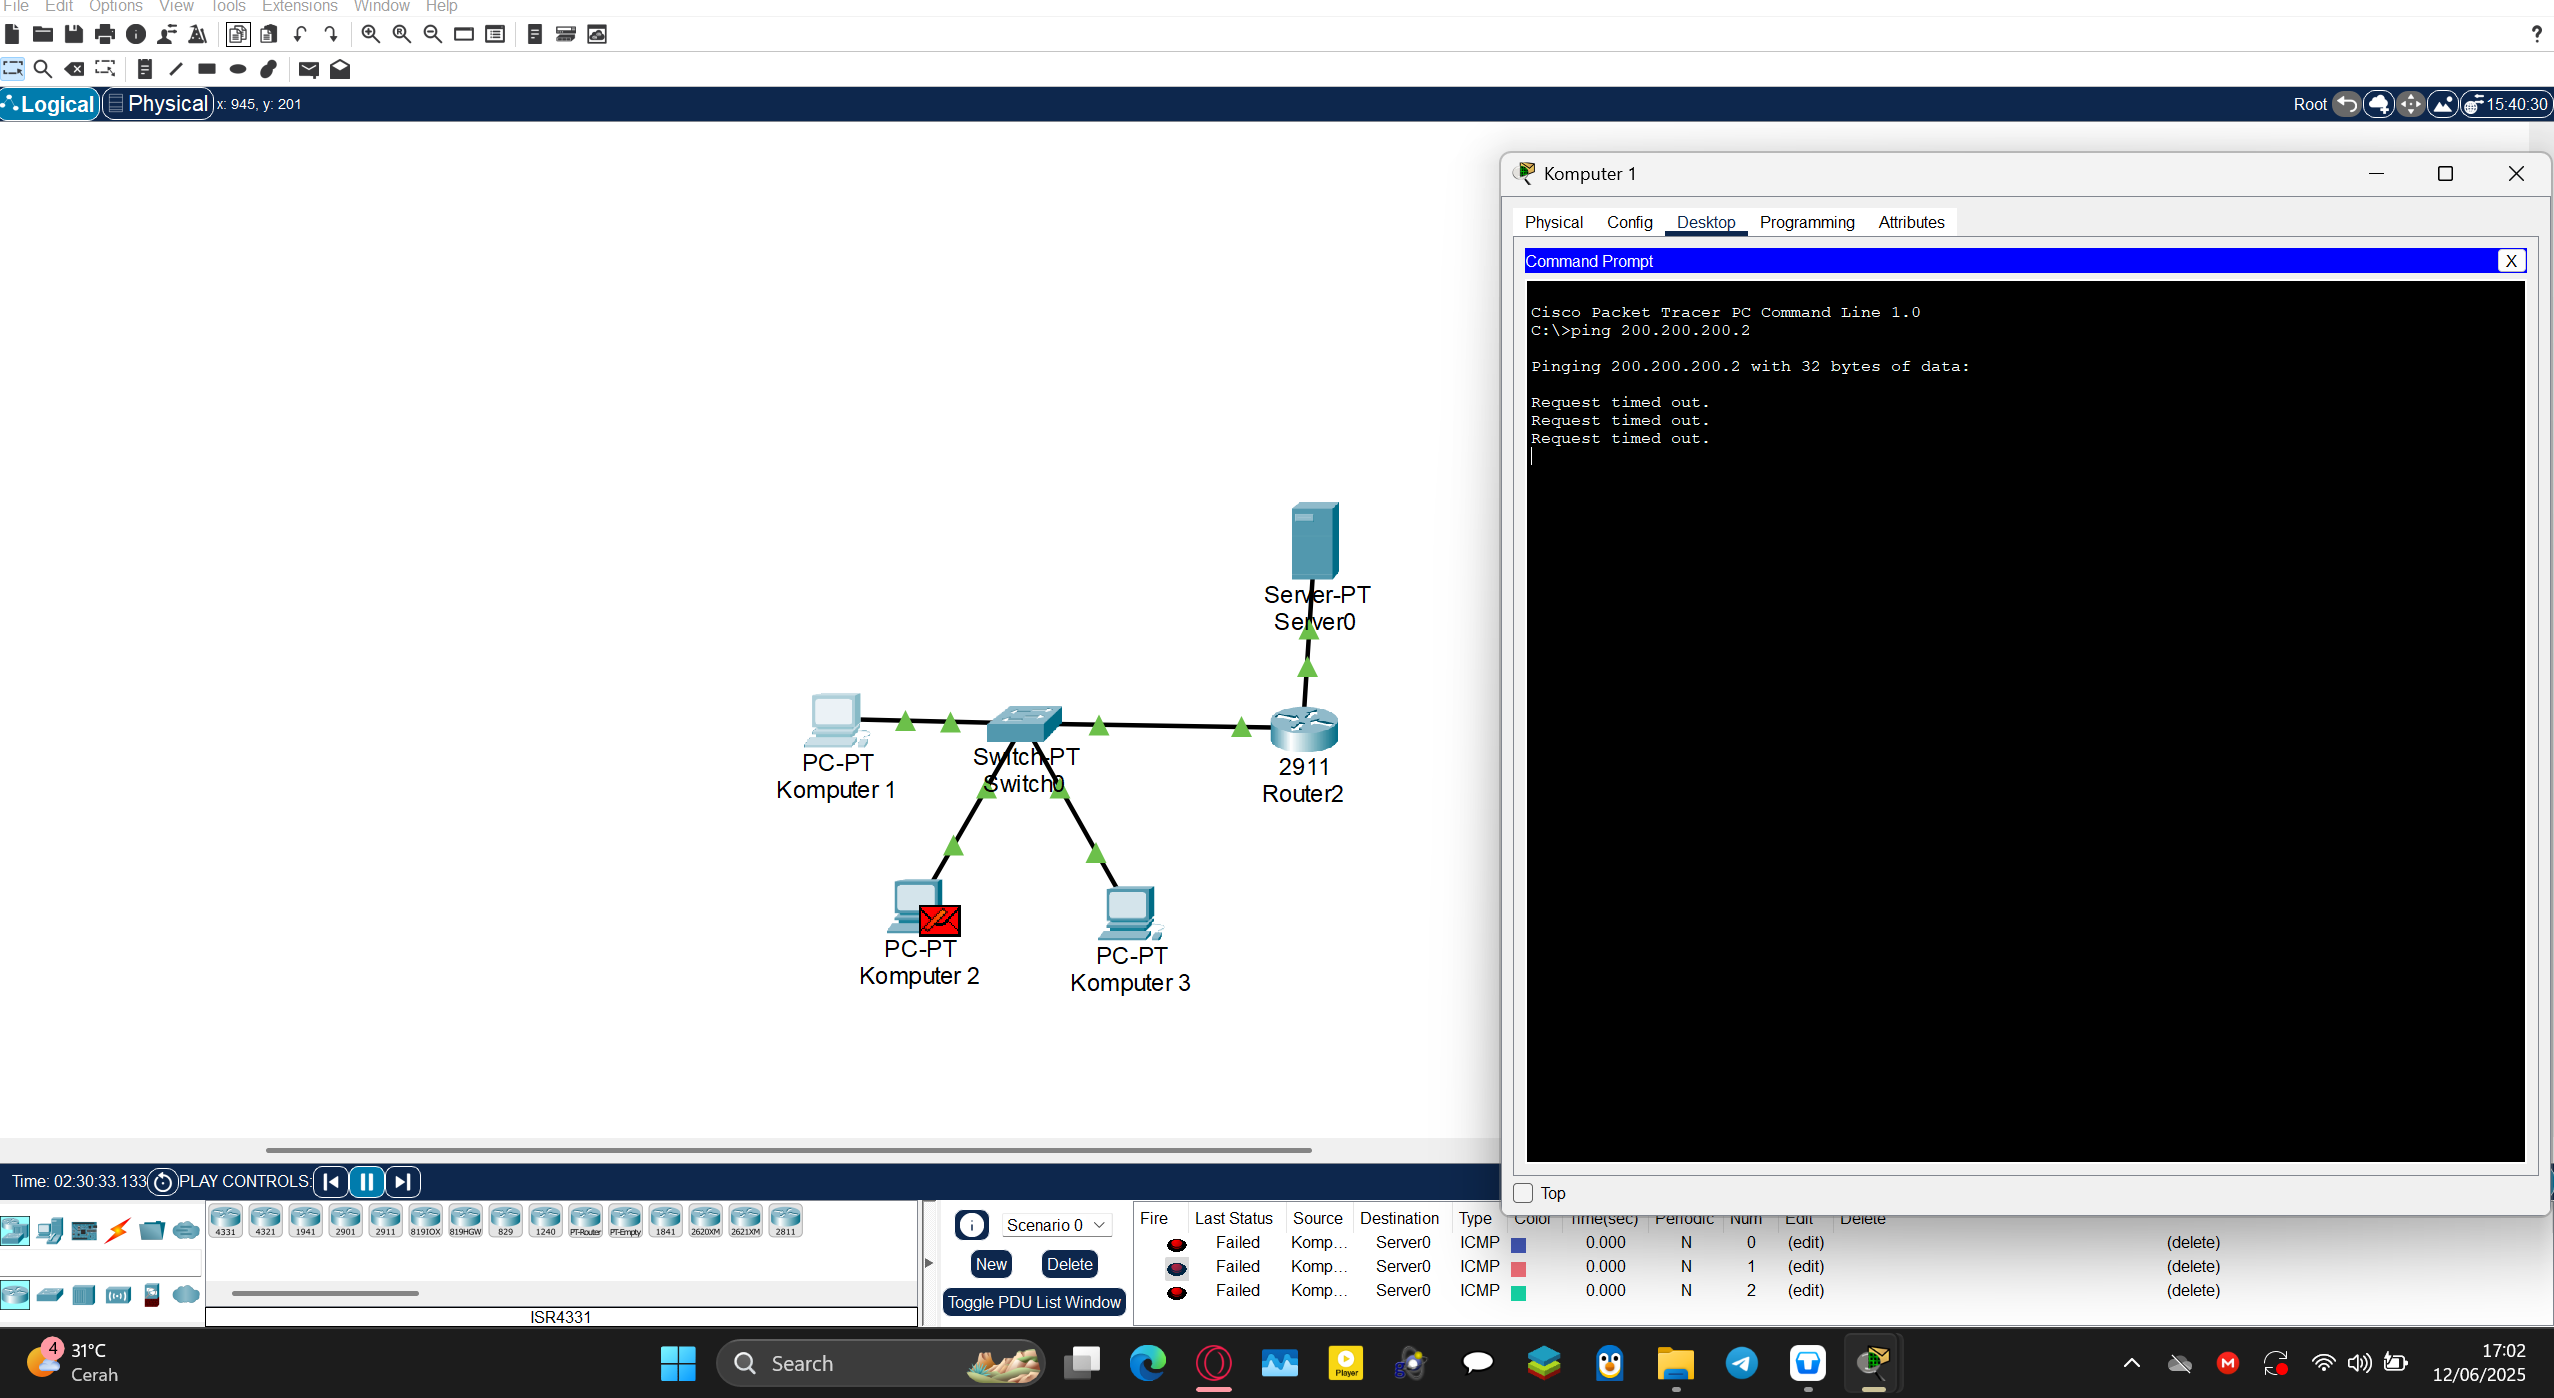
\includegraphics[width=0.8\linewidth]{P1/img/26.png}
        \caption{}
        \label{fig:gambar4}
    \end{figure}
    \begin{figure}[H]
        \centering
        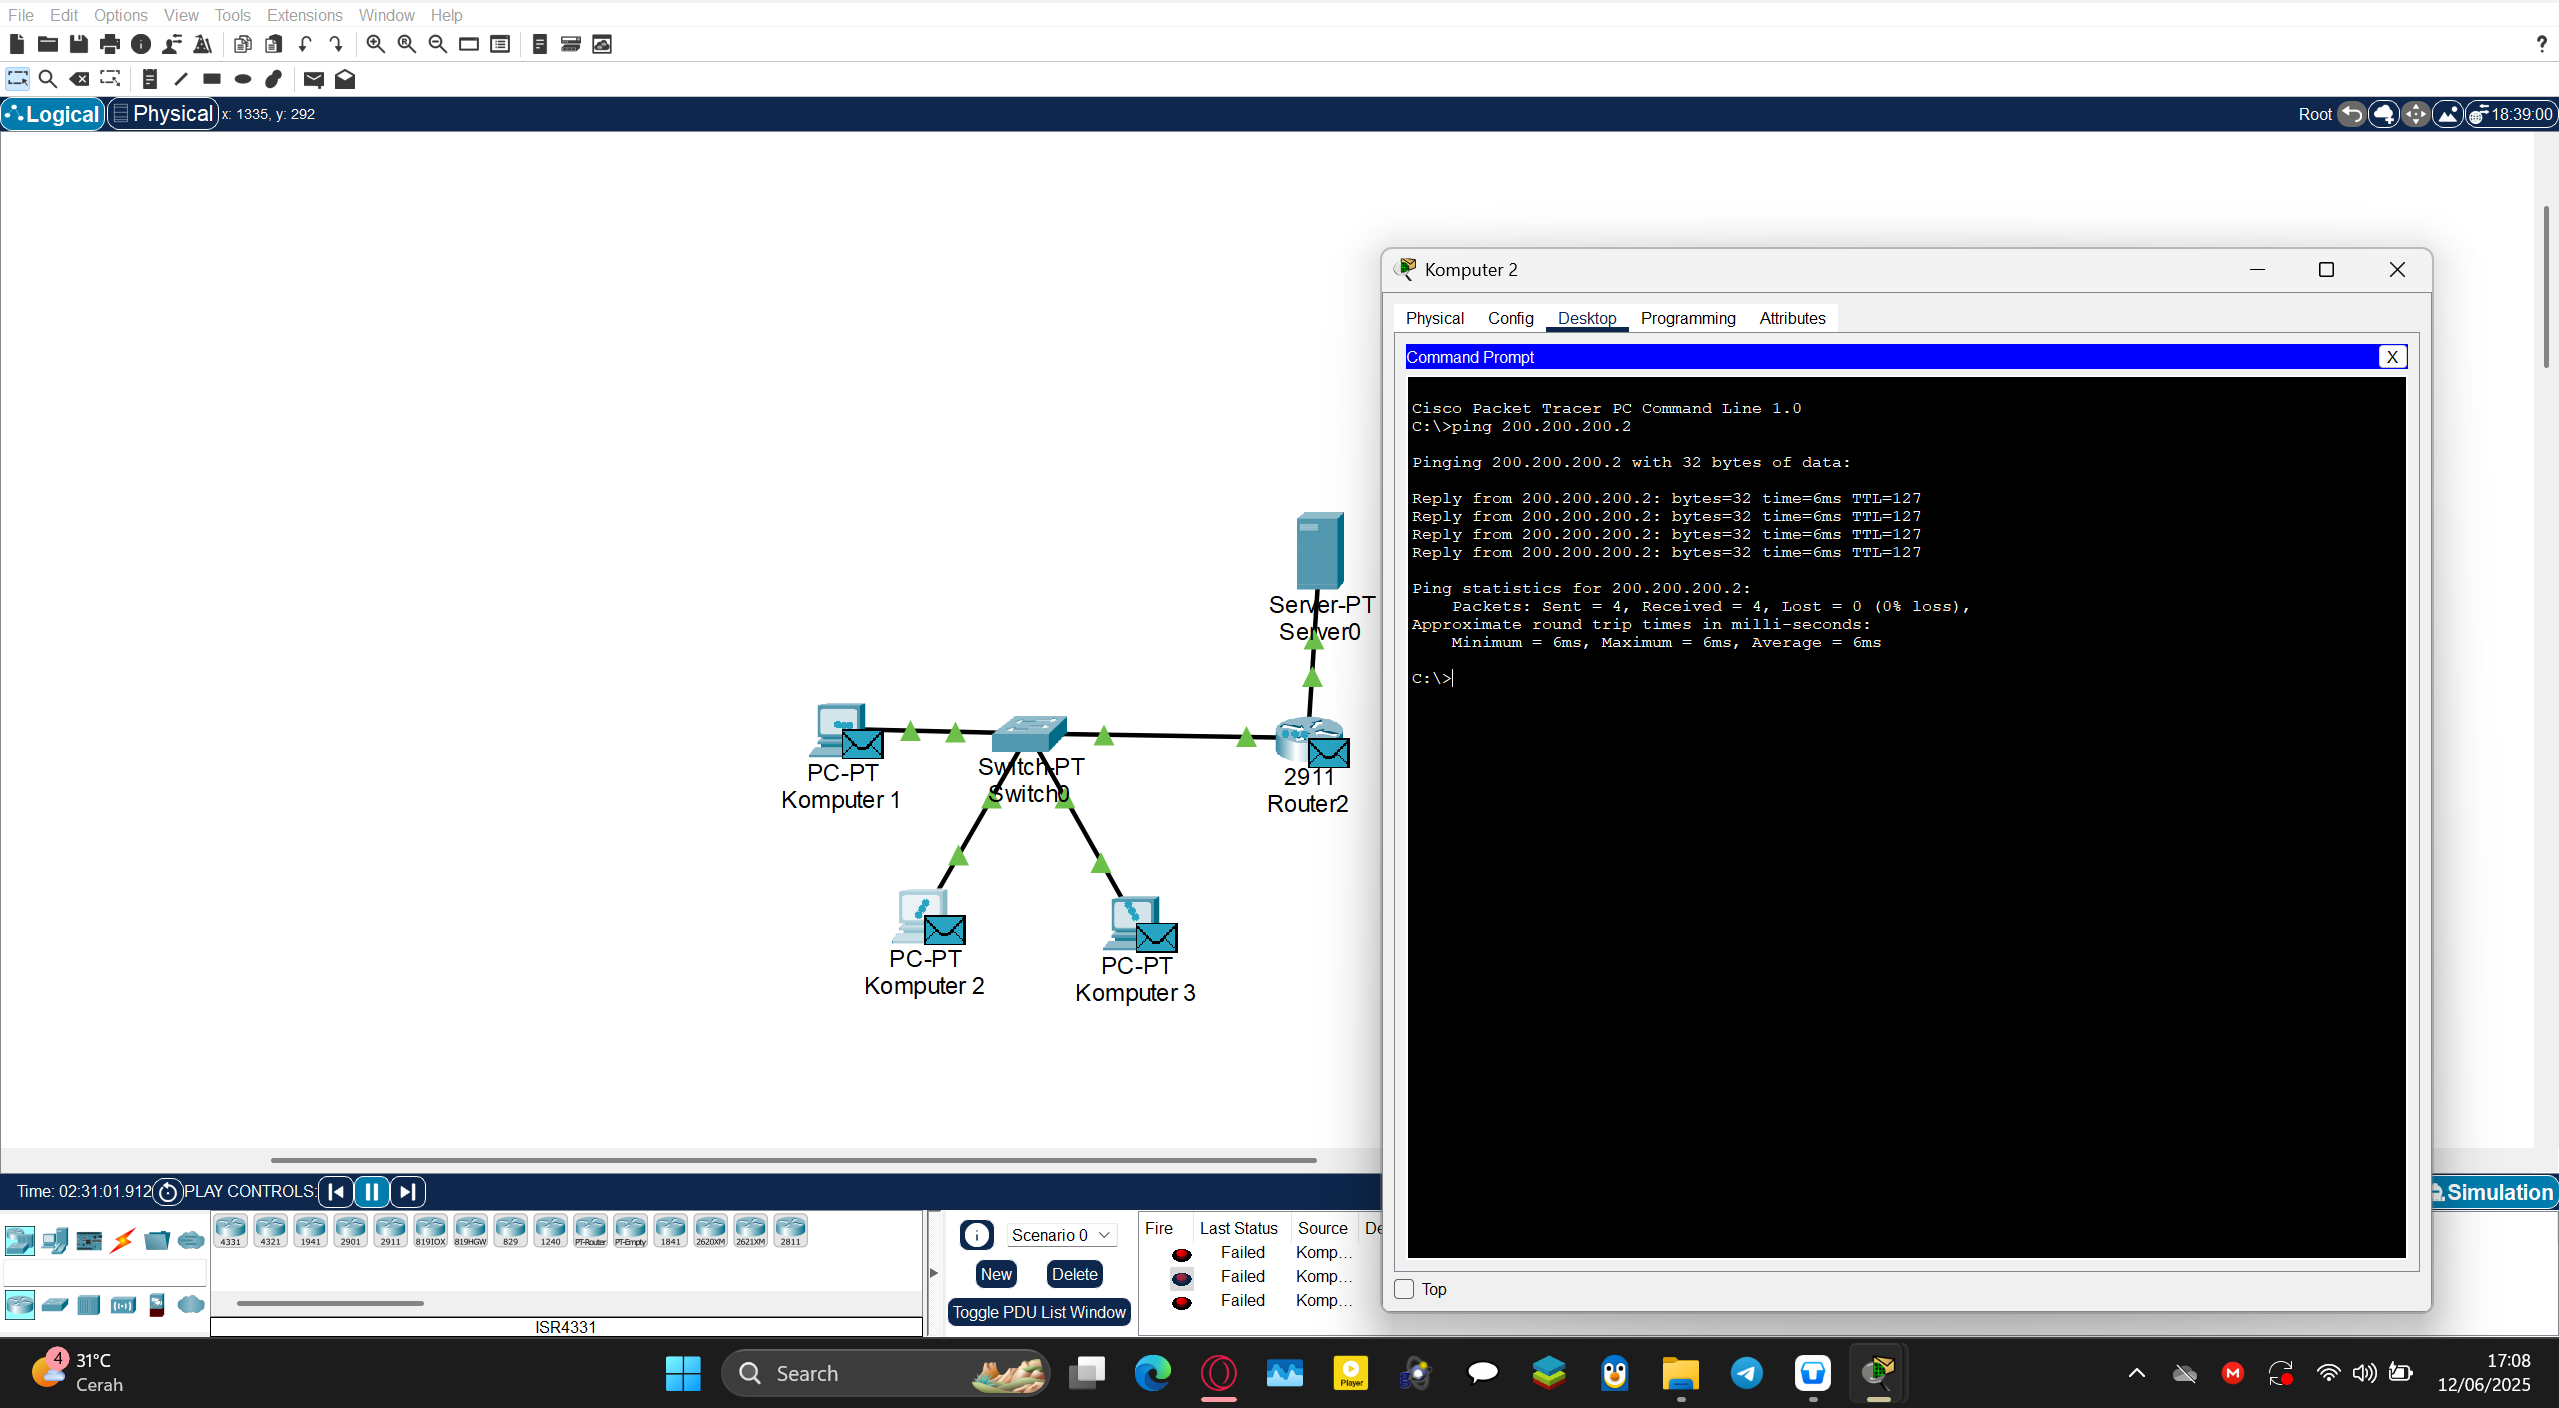
\includegraphics[width=0.8\linewidth]{P1/img/27.png}
        \caption{}
        \label{fig:gambar4}
    \end{figure}
    \begin{figure}[H]
        \centering
        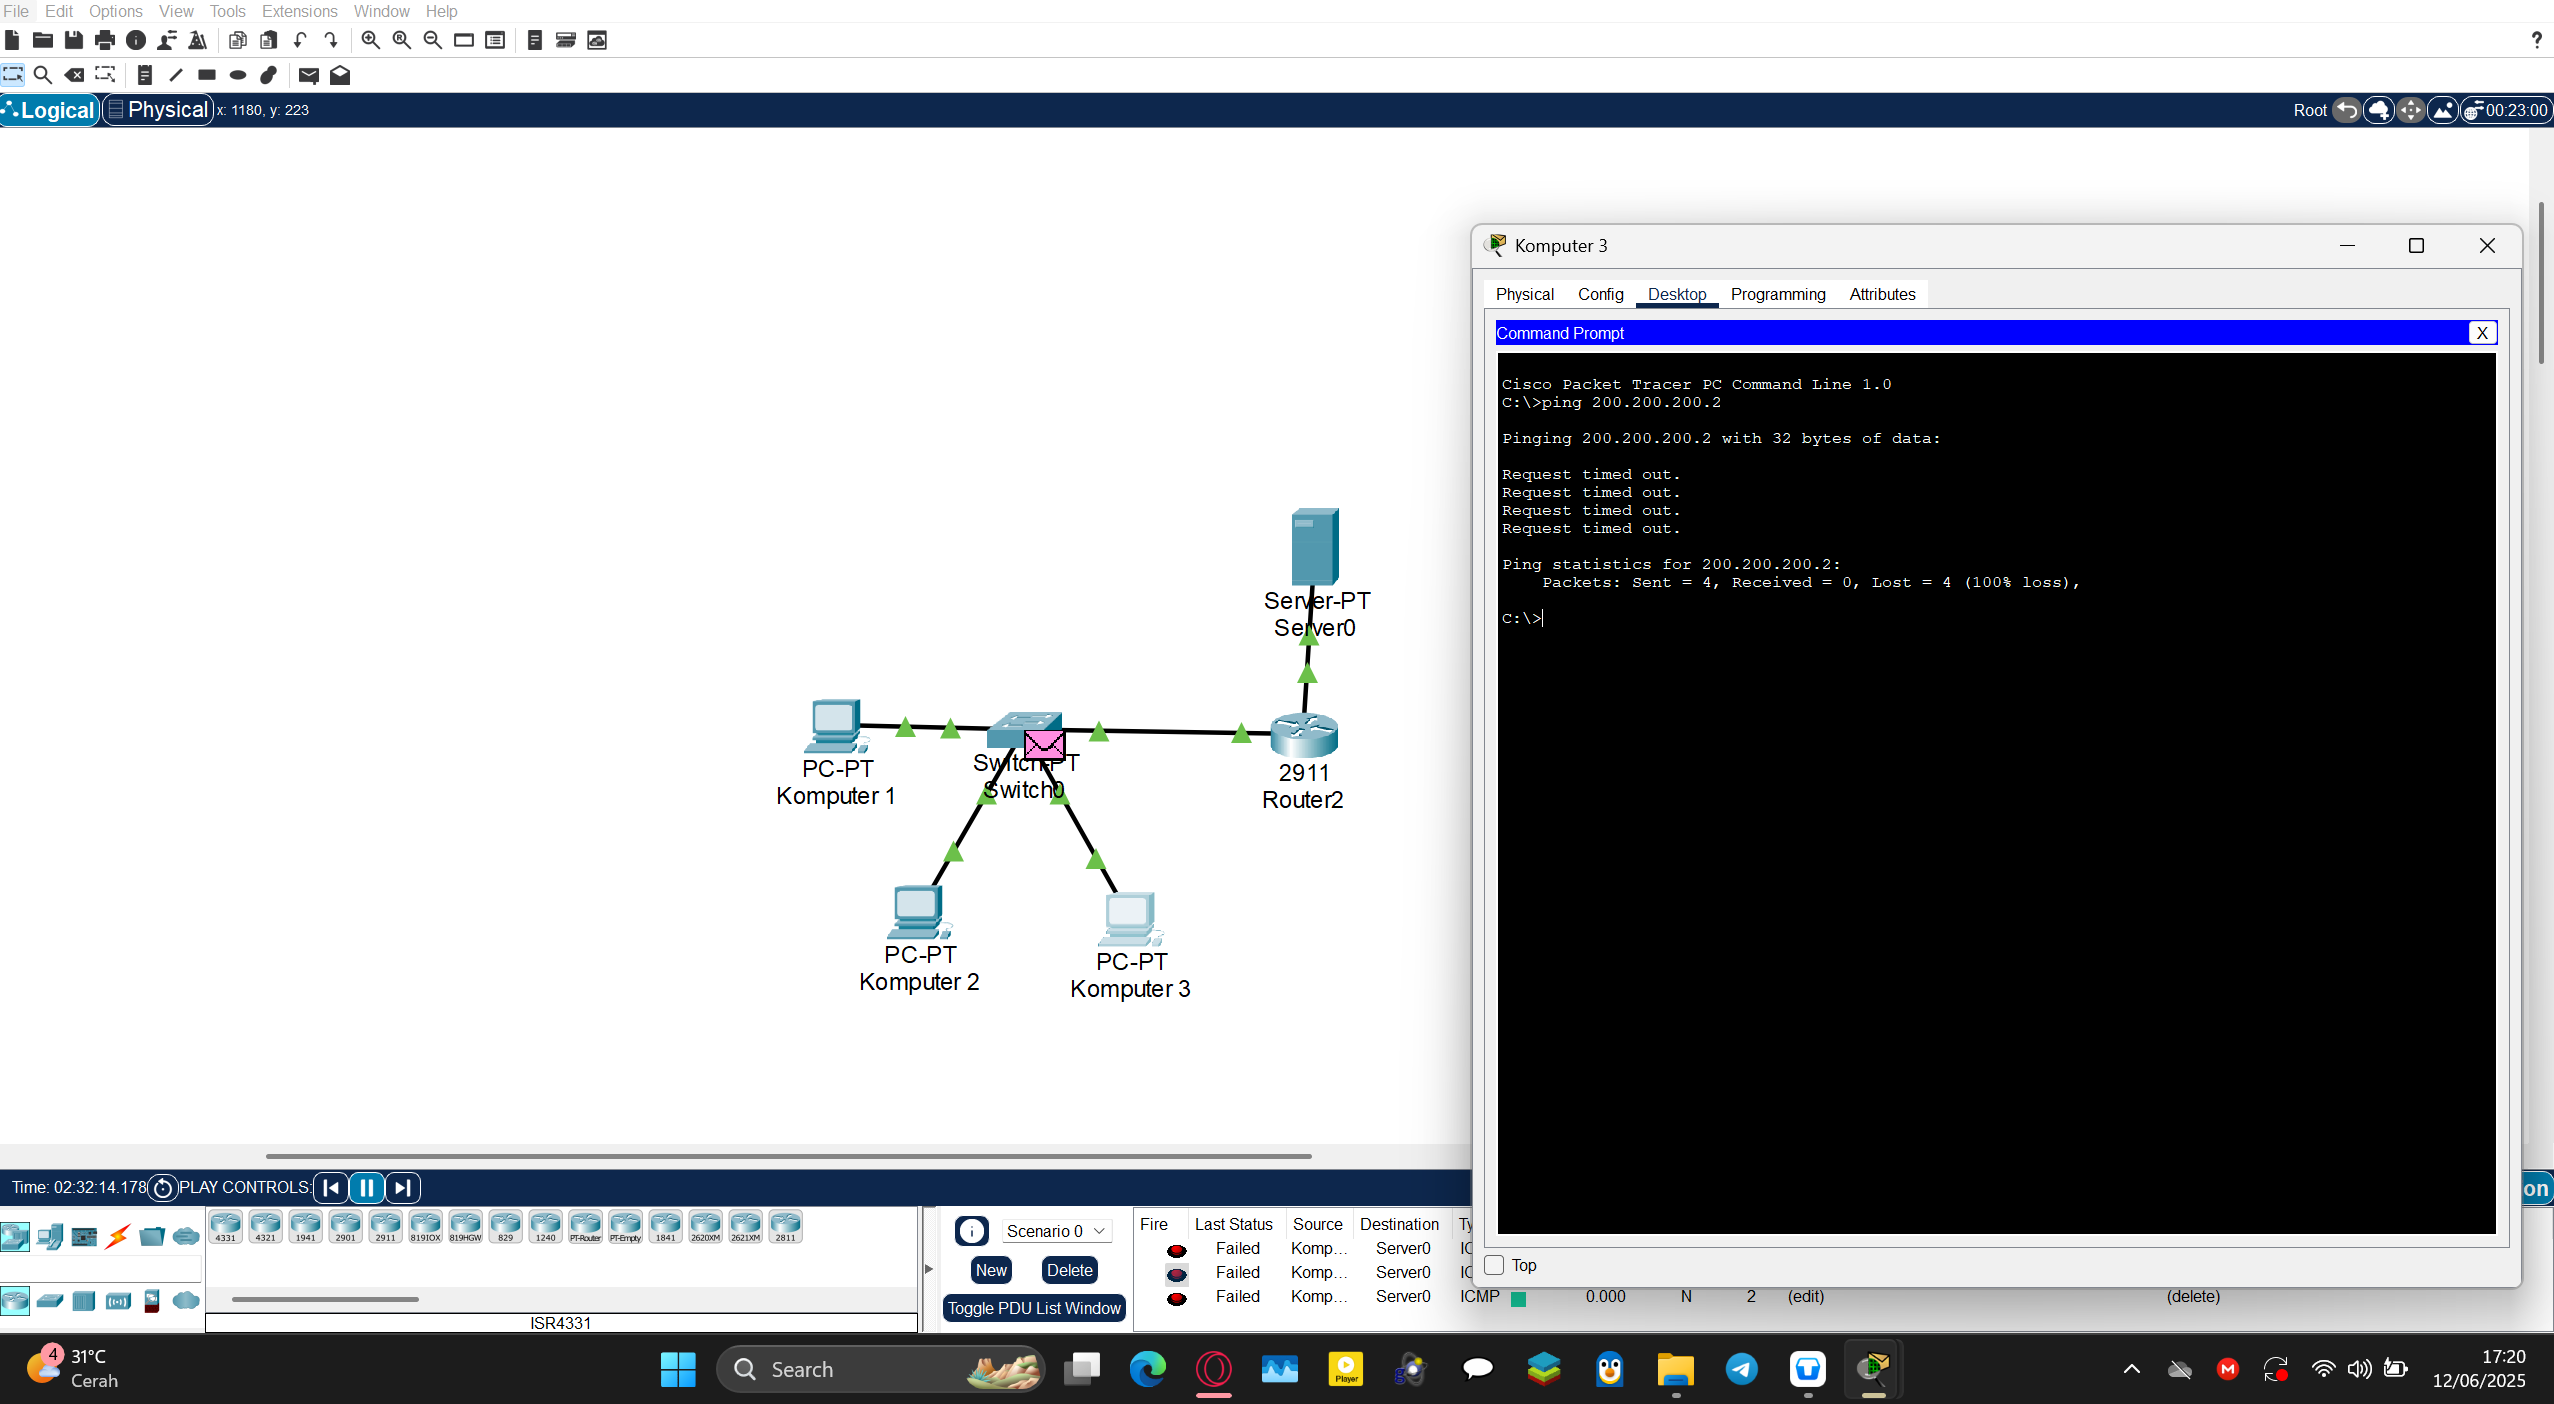
\includegraphics[width=0.8\linewidth]{P1/img/28.png}
        \caption{}
        \label{fig:gambar4}
    \end{figure}
    
\end{enumerate}

\section{Kesimpulan}
Berdasarkan praktikum yang telah dilakukan, dapat disimpulkan bahwa bahwa NAT berhasil memberikan akses internet ke jaringan lokal dengan satu IP publik, sementara firewall efektif dalam menyaring lalu lintas sesuai kebijakan yang ditentukan. Praktikum ini memberikan pemahaman praktis mengenai pentingnya penerapan kebijakan keamanan dan pengelolaan alamat IP dalam infrastruktur jaringan modern.

\section{Lampiran}
\subsection{Dokumentasi saat praktikum}
\begin{figure}[H]
        \centering
        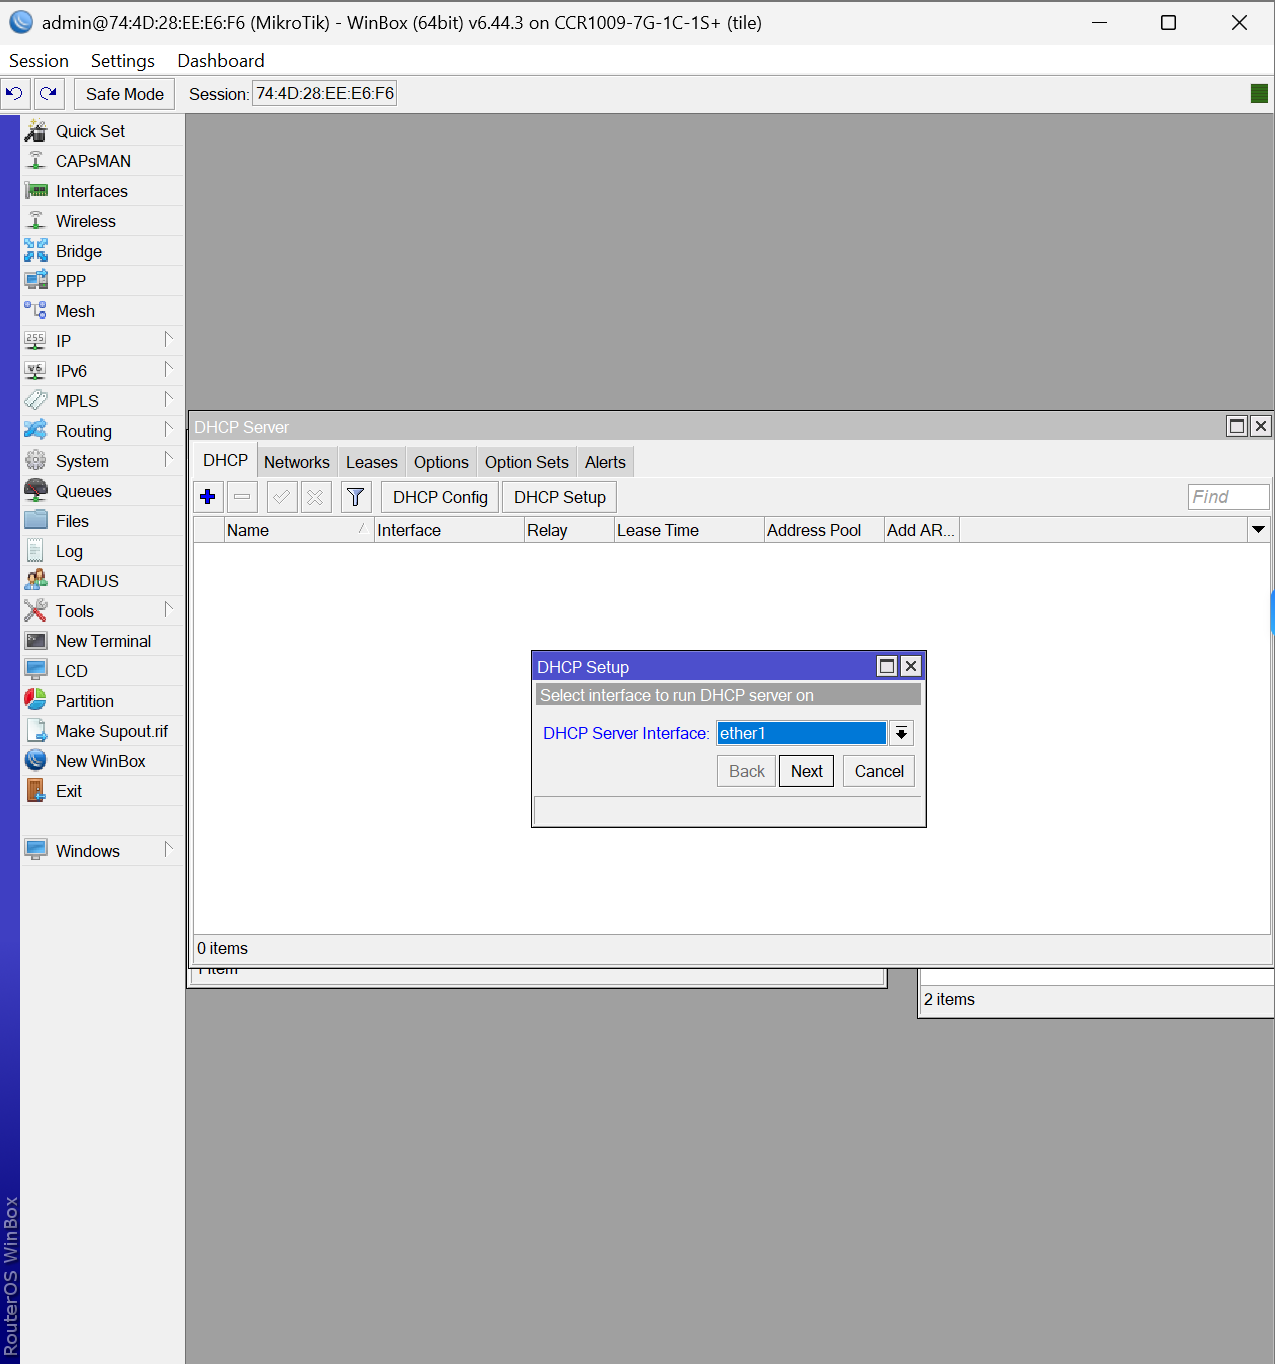
\includegraphics[width=0.5\linewidth]{P1/img/7.png}
        \caption{Dokumentasi}
        \label{fig:gambar1}
    \end{figure}

    \begin{figure}[H]
        \centering
        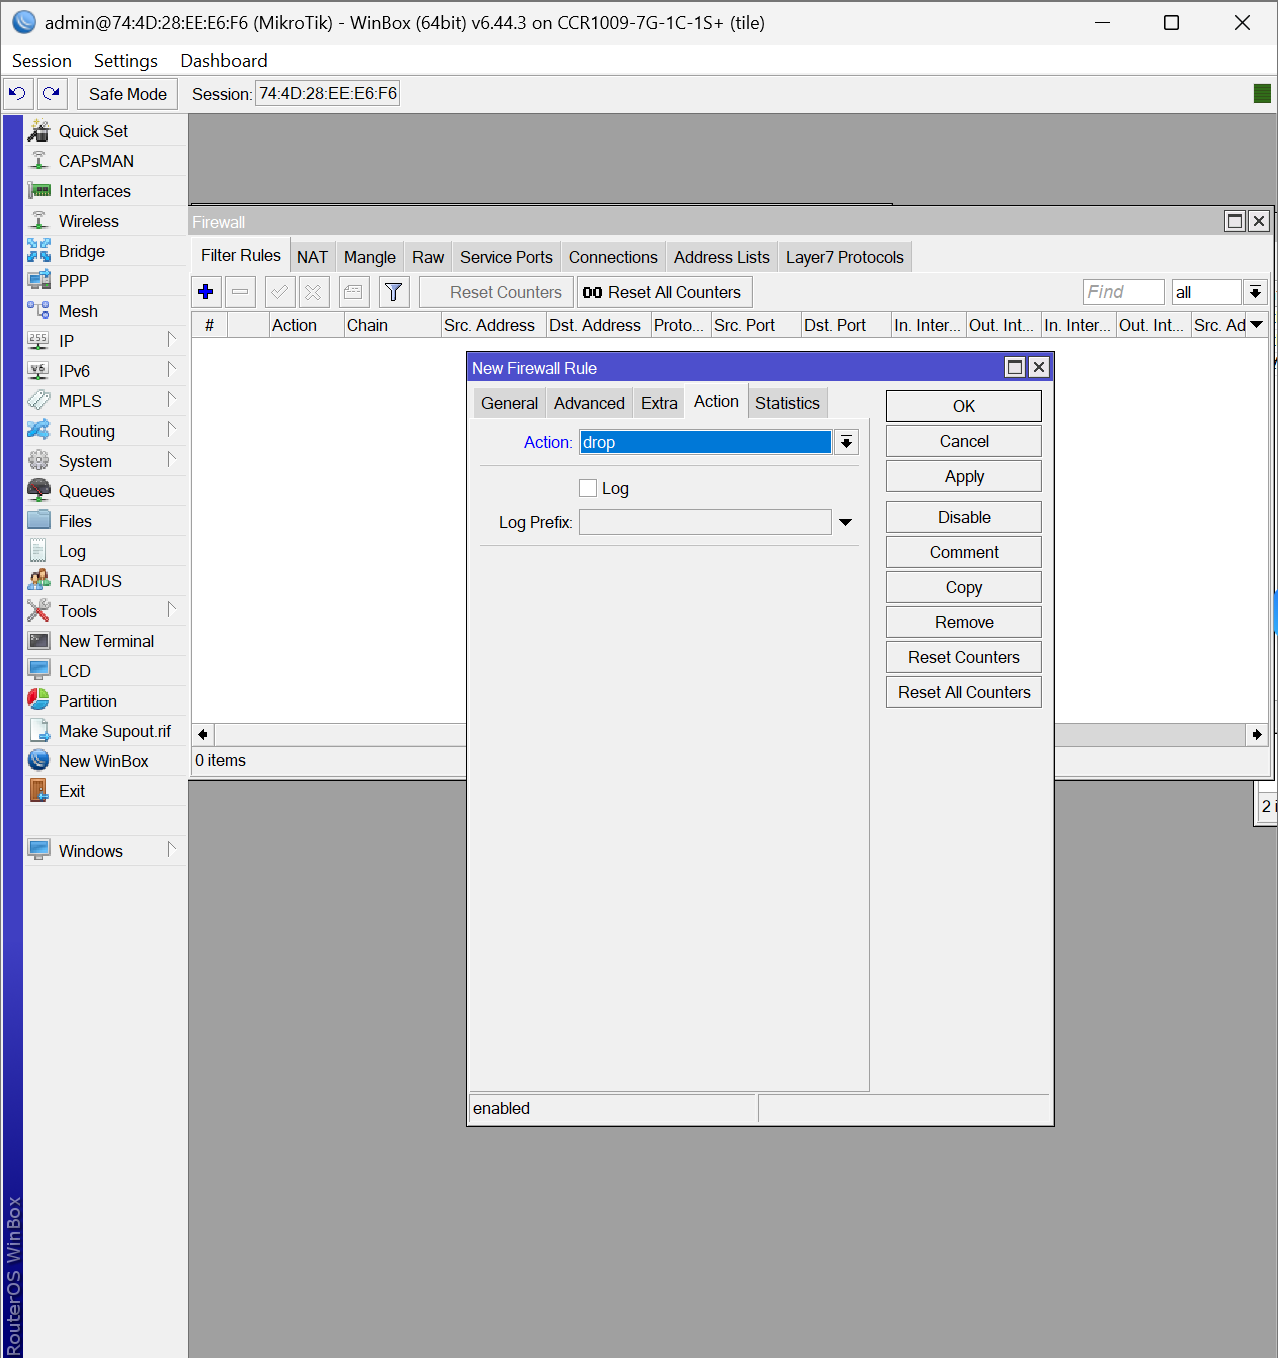
\includegraphics[width=0.5\linewidth]{P1/img/15}
        \caption{Dokumentasi}
        \label{fig:gambar1}
    \end{figure}

    \begin{figure}[H]
        \centering
        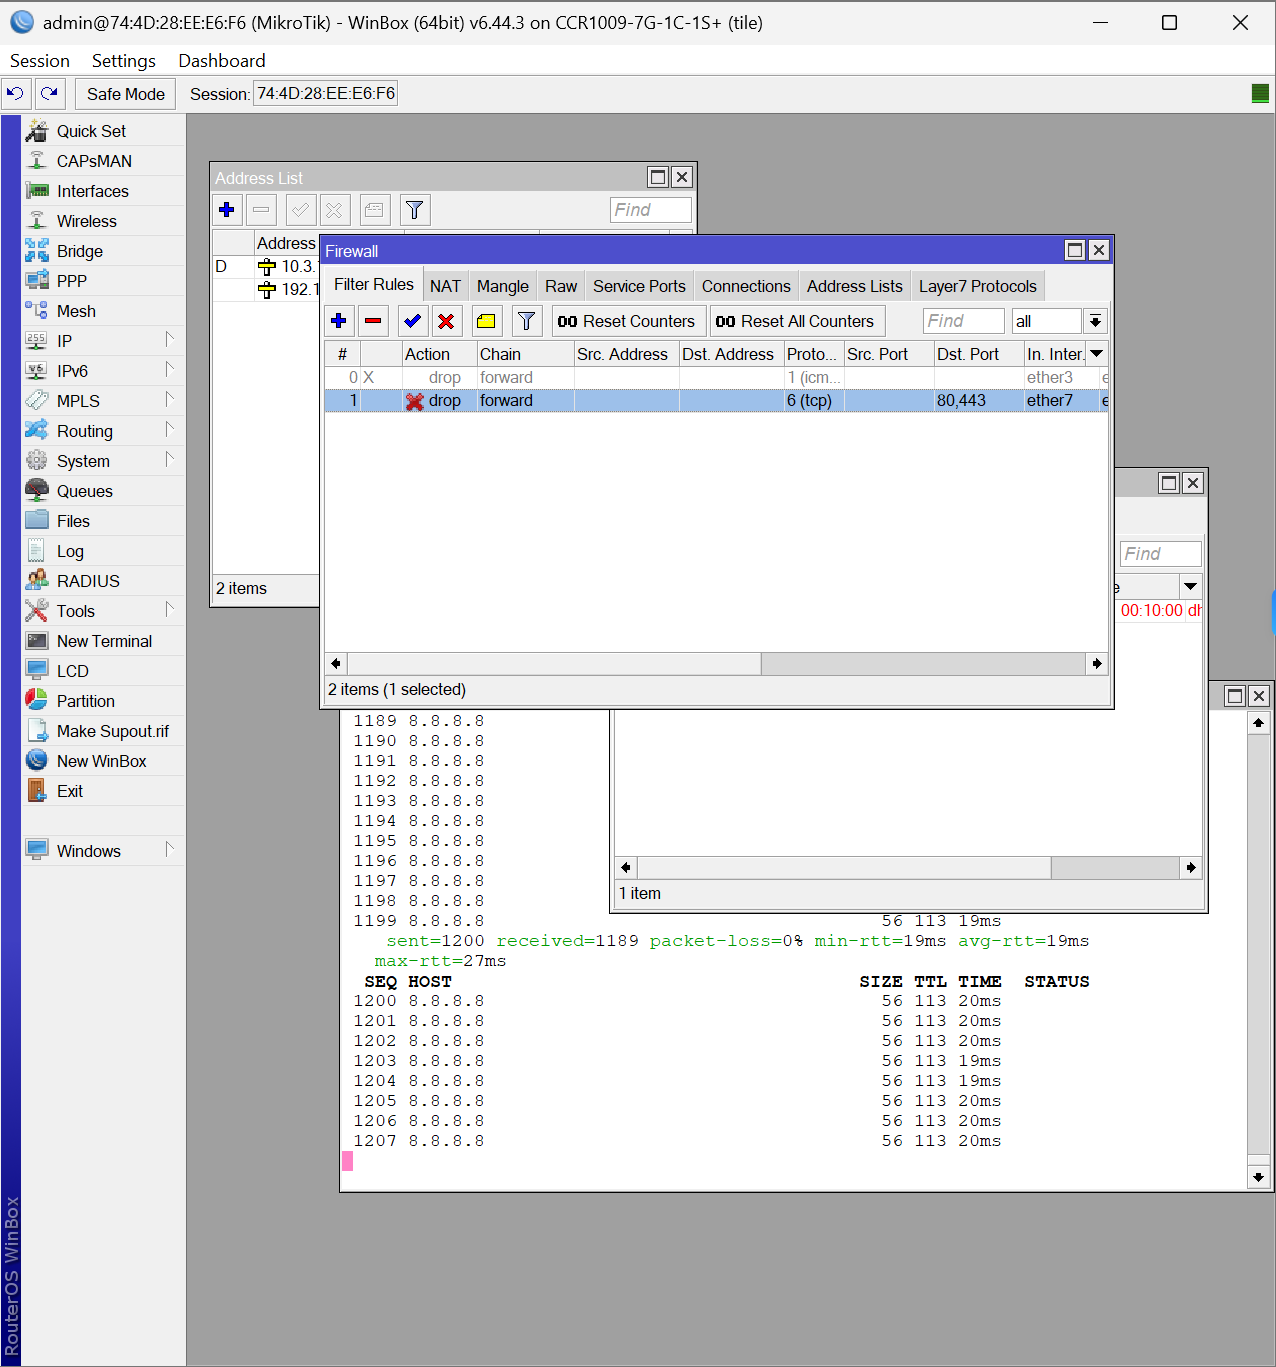
\includegraphics[width=0.5\linewidth]{P1/img/20.png}
        \caption{Dokumentasi}
        \label{fig:gambar1}
    \end{figure}

